
\section[Глава 1]{Глава 1. Методы молекулярного и интегративного модели­рования в структурной биологии.}
\subsection{Методы моделирования: возможности и ограничения}

\begin{frame}%[shrink=50]
\frametitle{Задача моделирования биомолекул}
%Слайд перутц, вайнштейн, Бернал, Улам
%Моделирование vs simulations
\centering
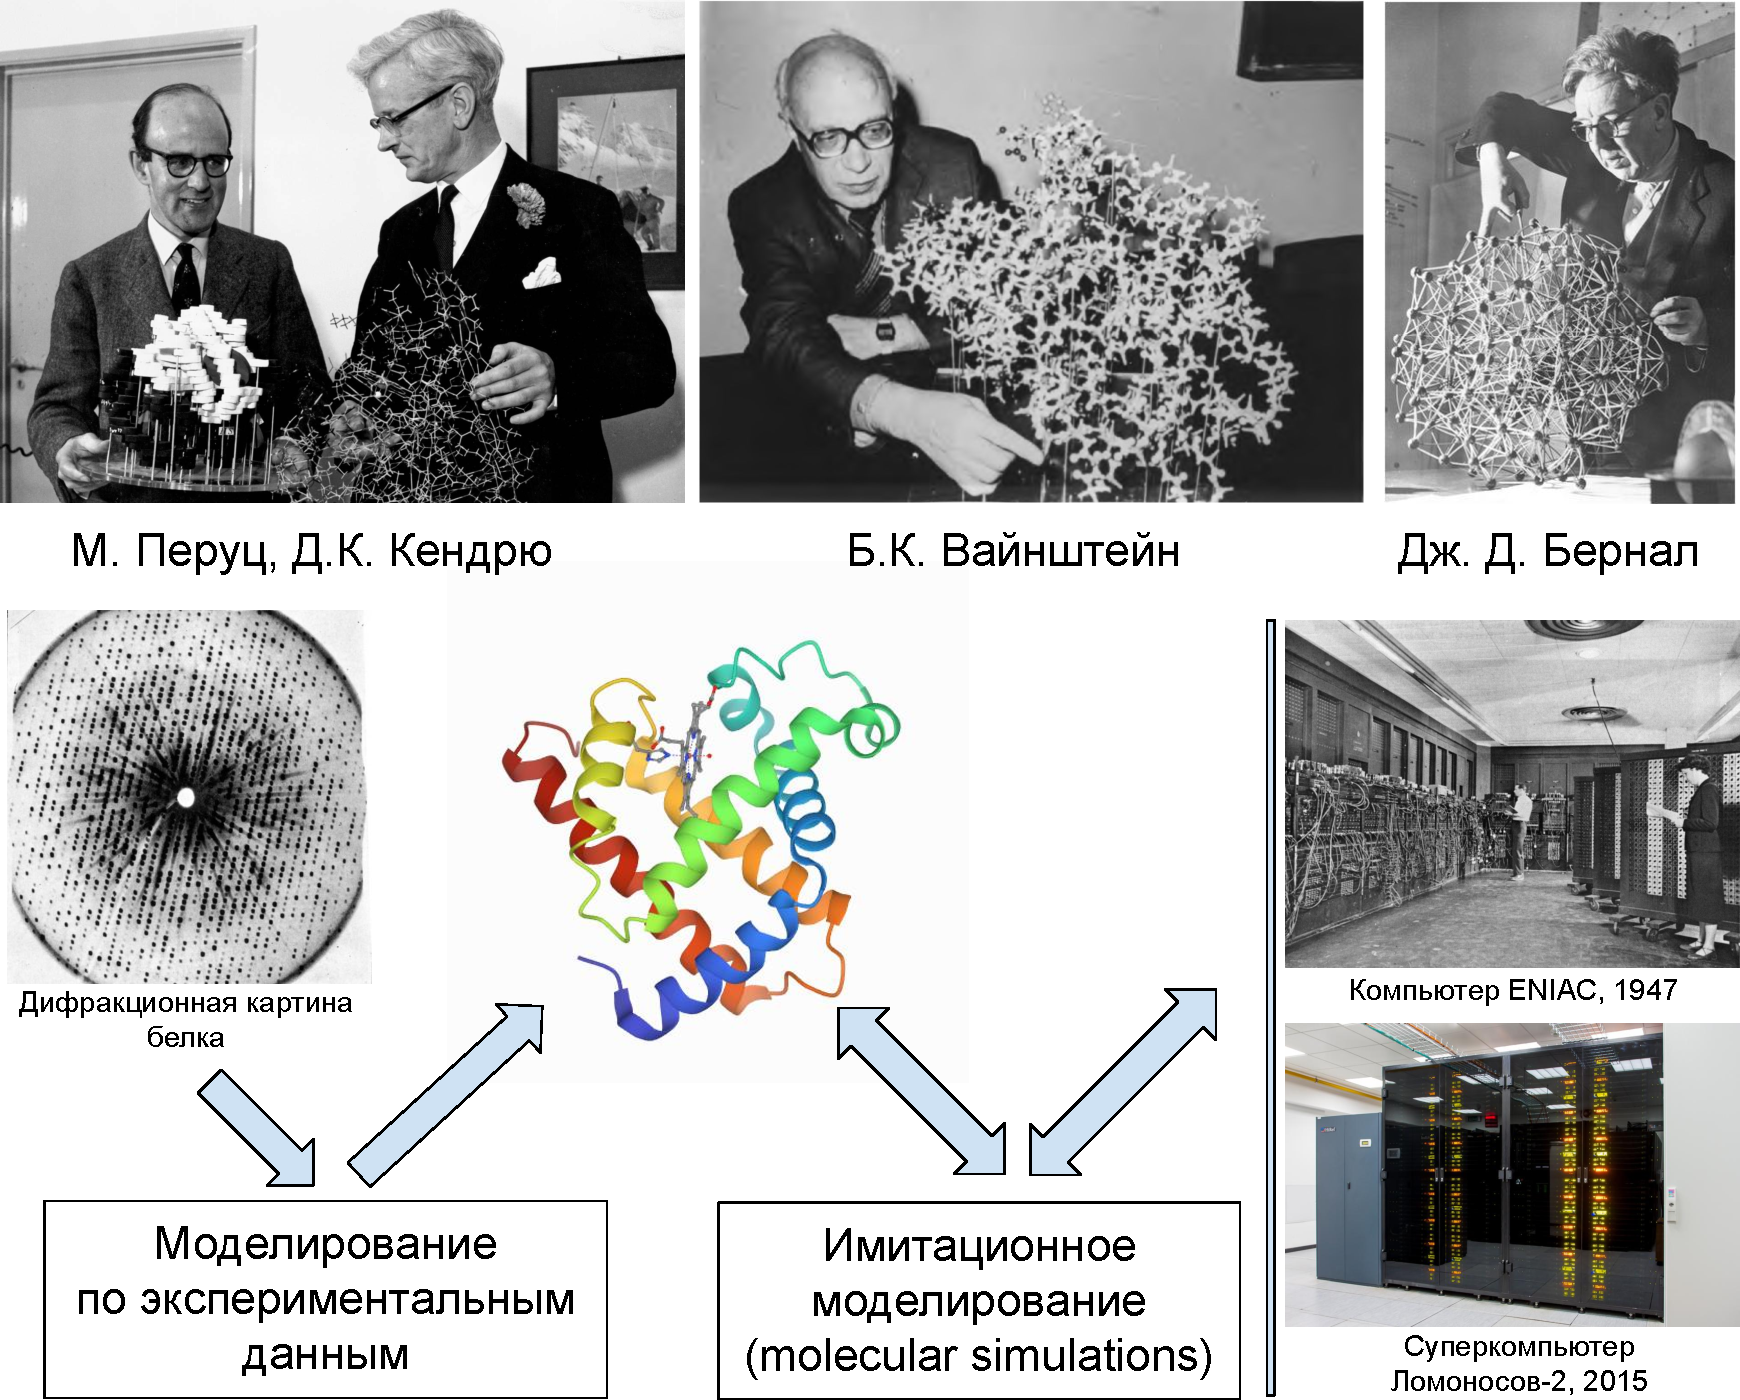
\includegraphics[height=0.85\textheight]{Presentation/images/s1} % окружение figure не требуется
% \begin{columns}
% \begin{column}{0.5\textwidth}
%    some text here some text here some text here some text here some text here
% \end{column}
% \begin{column}{0.5\textwidth}  %%<--- here
%     \begin{center}
%     \begin{itemize}
%         \item Проблема 1 \footnotemark
%         \item Проблема 2
%         \item Проблема 3
%     \end{itemize}
%      \end{center}
% \end{column}
% \end{columns}
% \footnotetext[1]{afjalfjkas}
\note{Изложение сутевой части работы начну с принципиального обсуждения методов и подходов моделирования биомакромолекул. Молекулярное моделирование является одними из важных способов изучения и познания живых систем. На слайде изображен ряд основоположников структурной биологии с физичкскими моделями молекул в руках в эпоху, когда персональные компьютеры еще не были распространены. Уже тогда было понятно, что методы моделирования могут быть подразделены на две группы. В одном случае задача сводится к построению пространственной модели расположения атомов, удовлетворящей наблюдаемым экспериментальным данным (например, ренгеновской дифракции). В другом случае, называемом имитационным моделированием, расположение атомов рассчитывается на основе вычисления внутри- и межмолекулярных взаимодействий между атомами. Развитие компьютеров активно способствовало разработке таких подходов, которые
позволяют рассмотривать в том числе и динамику биомолекул. (1.5-5)

}

\end{frame}


\begin{frame}
\frametitle{Методы молекулярной механики и динамики}
\underline{Полноатомное приближение}
  \begin{small}
   $$ U(\{\vec{r}_i\})= \sum_{bonds} \frac{1}{2} k_b (l-l_0)^2  + \sum_{angels} \frac{1}{2}k_\theta (\theta - \theta_0)^2 + \sum_{torsions} \frac{1}{2} V_n [1+\cos({n\varphi-\varphi_0})] + $$
   $$ \sum_{impropers} \frac{1}{2} k_\gamma (\gamma-\gamma_0)^2 + \sum_{j+1}^{N-1} \sum_{i=j+1}^{N} \Bigg\{ 4\epsilon_{ij} \Bigg[\Big(\frac{\sigma_{ij}}{r_{ij}}\Big)^{12} - \Big(\frac{\sigma_{ij}}{r_{ij}}\Big)^6\Bigg] + \frac{q_iq_j}{4\pi \epsilon_0 r_{ij}} \Bigg\} f_{ij} $$
   \end{small}%}

\begin{columns}
\begin{column}{0.45\textwidth}

%\scalebox{0.5}{%

   
     %\label{eq:p1_1:e1}
%\end{multline}}
   \centering
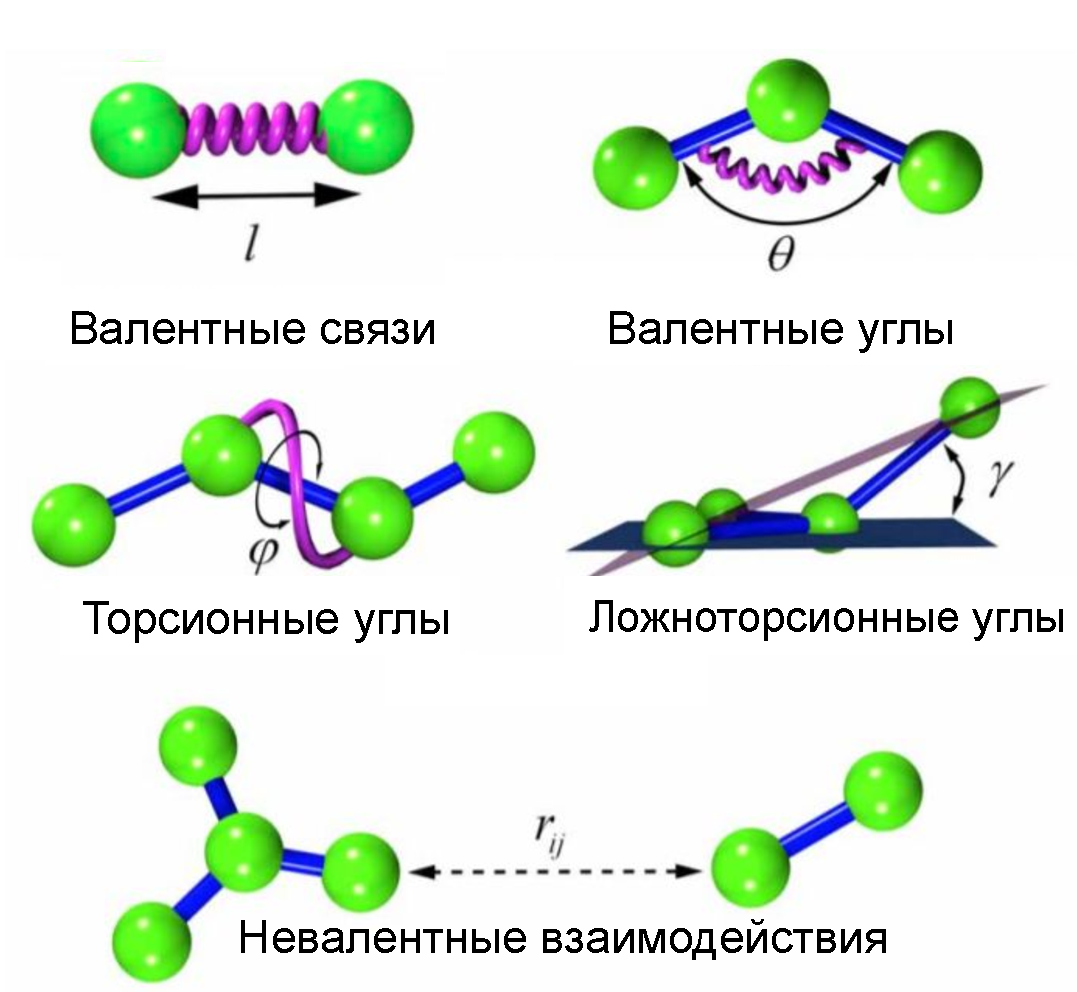
\includegraphics[width=1.0\textwidth]{s2l}
\end{column}
\begin{column}{0.45\textwidth}  %%<--- here
Численное решение уравнений движения ($\vec{F}=m\vec{a}$)
\ifdefined\HANDOUT
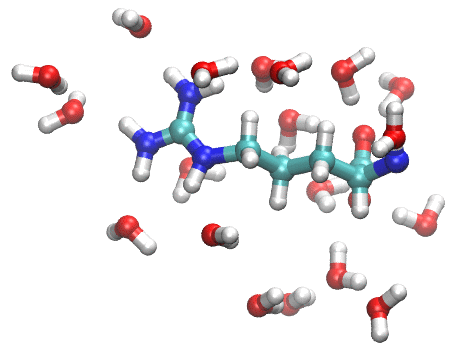
\includegraphics[width=0.9\linewidth]{arg/arg-50}
\else
\animategraphics[autoplay,loop,palindrome,width=0.9\linewidth]{10}{arg/arg-}{0}{50}
\fi
\end{column}
\end{columns}
\note{К таким методам при изучении биообъектов прежде всего относится метод молекулярной динамики. В методе МД физическая модель молекулы представляется в виде набора точечных атомов, взаимодействующим по законам классической механики Ньютона. Функция потенциальной энергии системы обычно задается аддитивным образом на основе комбинации элементарных функций и параметров, называемых силовым полем. В число элементарных взаимодействий входят зарядовые взаимодействия по закону Кулона, дисперсионные взаимодействия на основе потенциала Ван-дер-Ваальса, а также потенциалы, описывающие взаимодействия атомов, связанных химическими связями. Численное решение уравнений движения проводят с применением высокопроизводительного компьютерного и суперкомпьютерного оборудования. Современные вычислительные мощности позволяют достигать микросекундных, а иногда и миллисекундных времен моделирования. На таких временах проявляются термодинамические и статистические свойства молекулярных систем, появляется возможность исследовать различные функциональные процессы. (1.5-6.5)
}
\end{frame}


\begin{frame}
\frametitle{Методы молекулярной механики и динамики}
\underline{Огрубленное приближение} (пример ДНК)
  \begin{small}
   $$     F_k(\{\theta^k_j\})=F_0+\frac{1}{2}\sum_{i=1}^{6}\sum_{j=1}^{6}f_{ij}\Delta\theta^k_{i}\Delta\theta^k_{j}, \; \Delta\theta^k_{i}=(\theta^k_{i}-\hat{\theta}^k_{i}) $$
   \end{small}%}
\begin{columns}
\begin{column}{0.5\textwidth}

%\scalebox{0.5}{%

   
     %\label{eq:p1_1:e1}
%\end{multline}}
   \centering
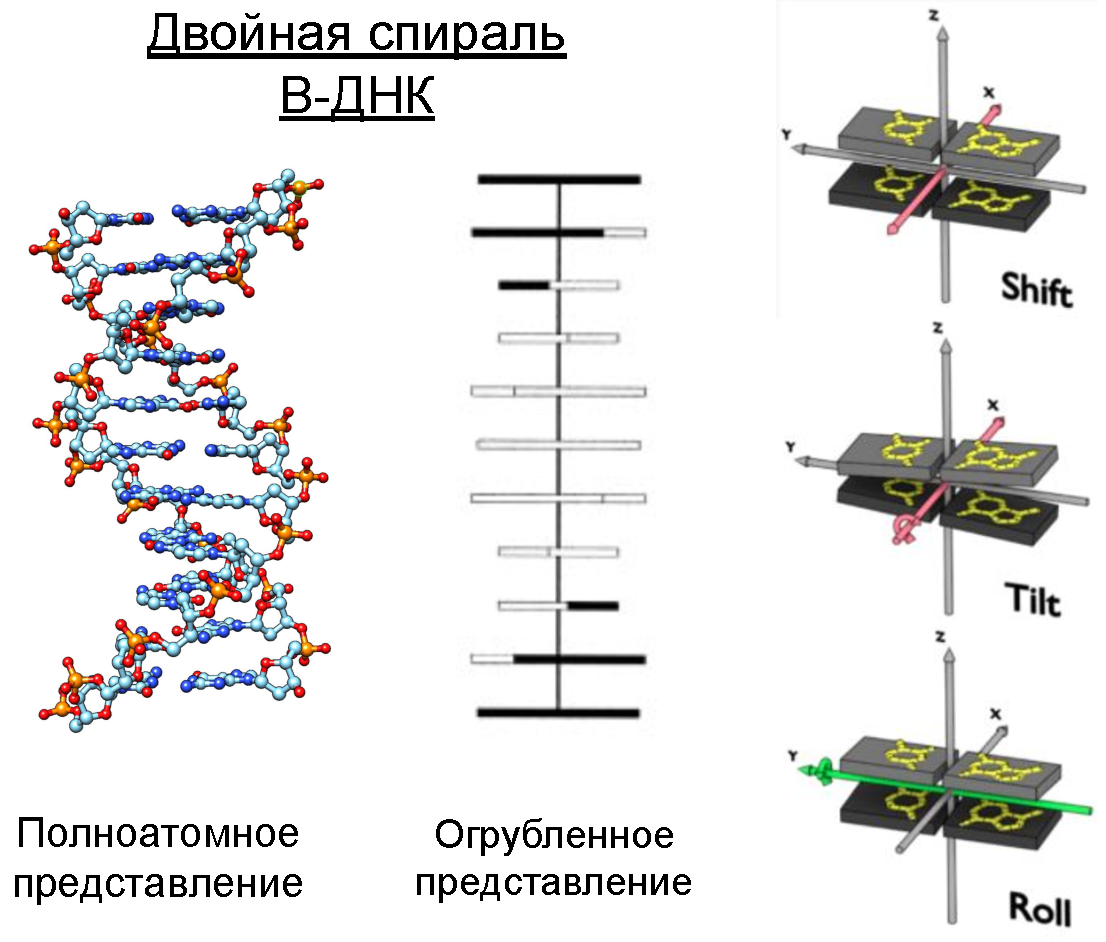
\includegraphics[width=1.0\textwidth]{s3l}
\end{column}
\begin{column}{0.5\textwidth}  %%<--- here
Применение метода Монте-Карло
\begin{center}
\ifdefined\HANDOUT
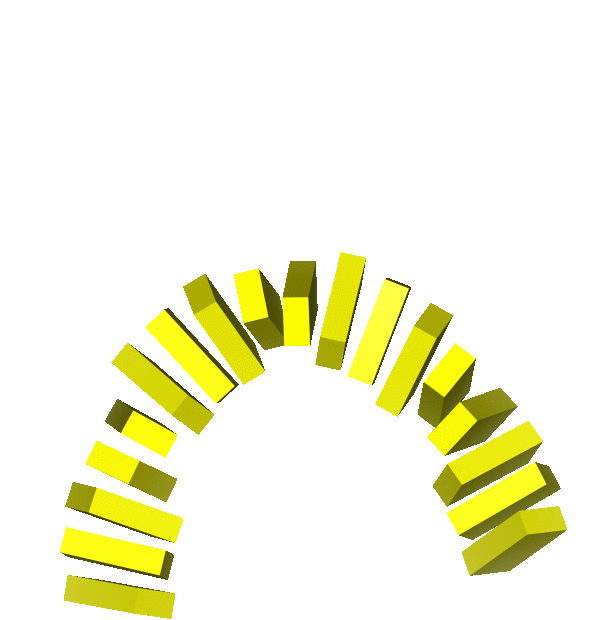
\includegraphics[width=0.8\linewidth]{DNA/DNAc-100}
\else
\animategraphics[autoplay,loop,palindrome,width=0.8\linewidth]{10}{DNA/DNAc-}{12}{125}
\fi
\end{center}
\end{column}
\end{columns}
\note{\footnotesize{
Свою нишу занимают и так называемые огрубленные подходы к моделированию. В этом случае целая группа атомов может быть представлена в виде некоторой механической единицы. Например, в случае ДНК пара оснований может быть представлена в виде прямоугольника, а функция потенциальной энергии задана как зависимость от взаимного расположения пар оснований. Такие упрощенные модели зачастую позволяют ускорить моделирование, а разумный выбор пространственных координат использовать более гибкие и эффективные подходы к моделированию, например, метод Монте-Карло. (1-7.5)}

}
\end{frame}


\begin{frame}
\frametitle{Проблемы моделирования биомакромолекулярных комплексов}
   {\Large Большой размер $\Longleftrightarrow$ Структурный полиморфизм}
\bigskip
    % \begin{enumerate}
        % \item один
        % \item два
        % \item три
    % \end{enumerate}
\begin{columns}[t]
\begin{column}{0.45\textwidth}
\underline{Экспериментальные ограничения}
 \begin{itemize}
        \item Сложность кристаллизации (РСА)
        \item Сложность деконволюции усредненного сигнала от набора конформаций
        \item Сложность детекции и обработки сигнала (ЯМР)
        \item Неустойчивость комплексов
    \end{itemize}
\end{column}
\begin{column}{0.55\textwidth}  %%<--- here
\underline{Вычислительные ограничения}
 \begin{itemize}
        \item Ограниченные времена моделирования
        \item Времена функциональной динамики комплексов существенно больше
        \item Ограниченная точность силовых полей
        \item Чувствительность конформаций комплексов к точности параметров моделирования
    \end{itemize}
\end{column}
\end{columns}

\note{\footnotesize{Несмотря на существенный прогресс как методов структурной биологии, так и методов вычислительной биофизики, в понимании структурно-динамической организации биомакромолекул имеется ряд затруднений. В особенности это относится к биомакромолекулярным комплексам.

Основных факторов, затрудняющих исследование структурной организации биомолекул, два -- это большой размер и динамический полиморфизм. При этом они взаимосвязаны - большие комплексы зачастую обладают богатым набором конформационных состояний, а отдельные домены могут относится к классу неупорядоченных белков.
В качестве яркого примера можно привести проблему описания упаковки ДНК в ядре эукариотических клеток, которая требует развития новых концептуальных походов на стыке полимерной физики и сруктурной биологии.

Размер и полиморфизм биомакромолекулярных комплексов перпятствует их эффективному изучению классическими методами структурной биологии (рентгеностурктурный анализ, ЯМР, крио-ЭМ).

Однако и моделирование их методами молекулярной динамики также затруднительно.
Осоновных проблемы здесь две. Во-первых, с ростом сложности молекулярной системы увеличиваются и времена функциональной динамики. Например, фолдинг белков проиходит обычно на субмиллисекундных и миллисекундных масштабах, а сборка ДНК-белкового комплекса нуклеосомы занимает уже десятки секунд. Расчеты необходимой длины не всегда достижимы при современном уровне развития вычислительной техники.
Вторая проблемя связана со сложностью задания силовых полей с нужной точностью. Небольшие неточности при задании атом-атомных потенциалов влияют сразу на большое количество взаимодействующих атомов и могут приводить к серьезным отклонениям в поведения системы.(2-9.5)

}}
\end{frame}

% \begin{frame}
% \frametitle{Виды экспериментальных данных о структуре и динамике биомолекул}

% \note{РСА, ЯМР,}
% \end{frame}

\subsection{Интегративные подходы}

\begin{frame}
\frametitle{Интегративные подходы}
   \centering
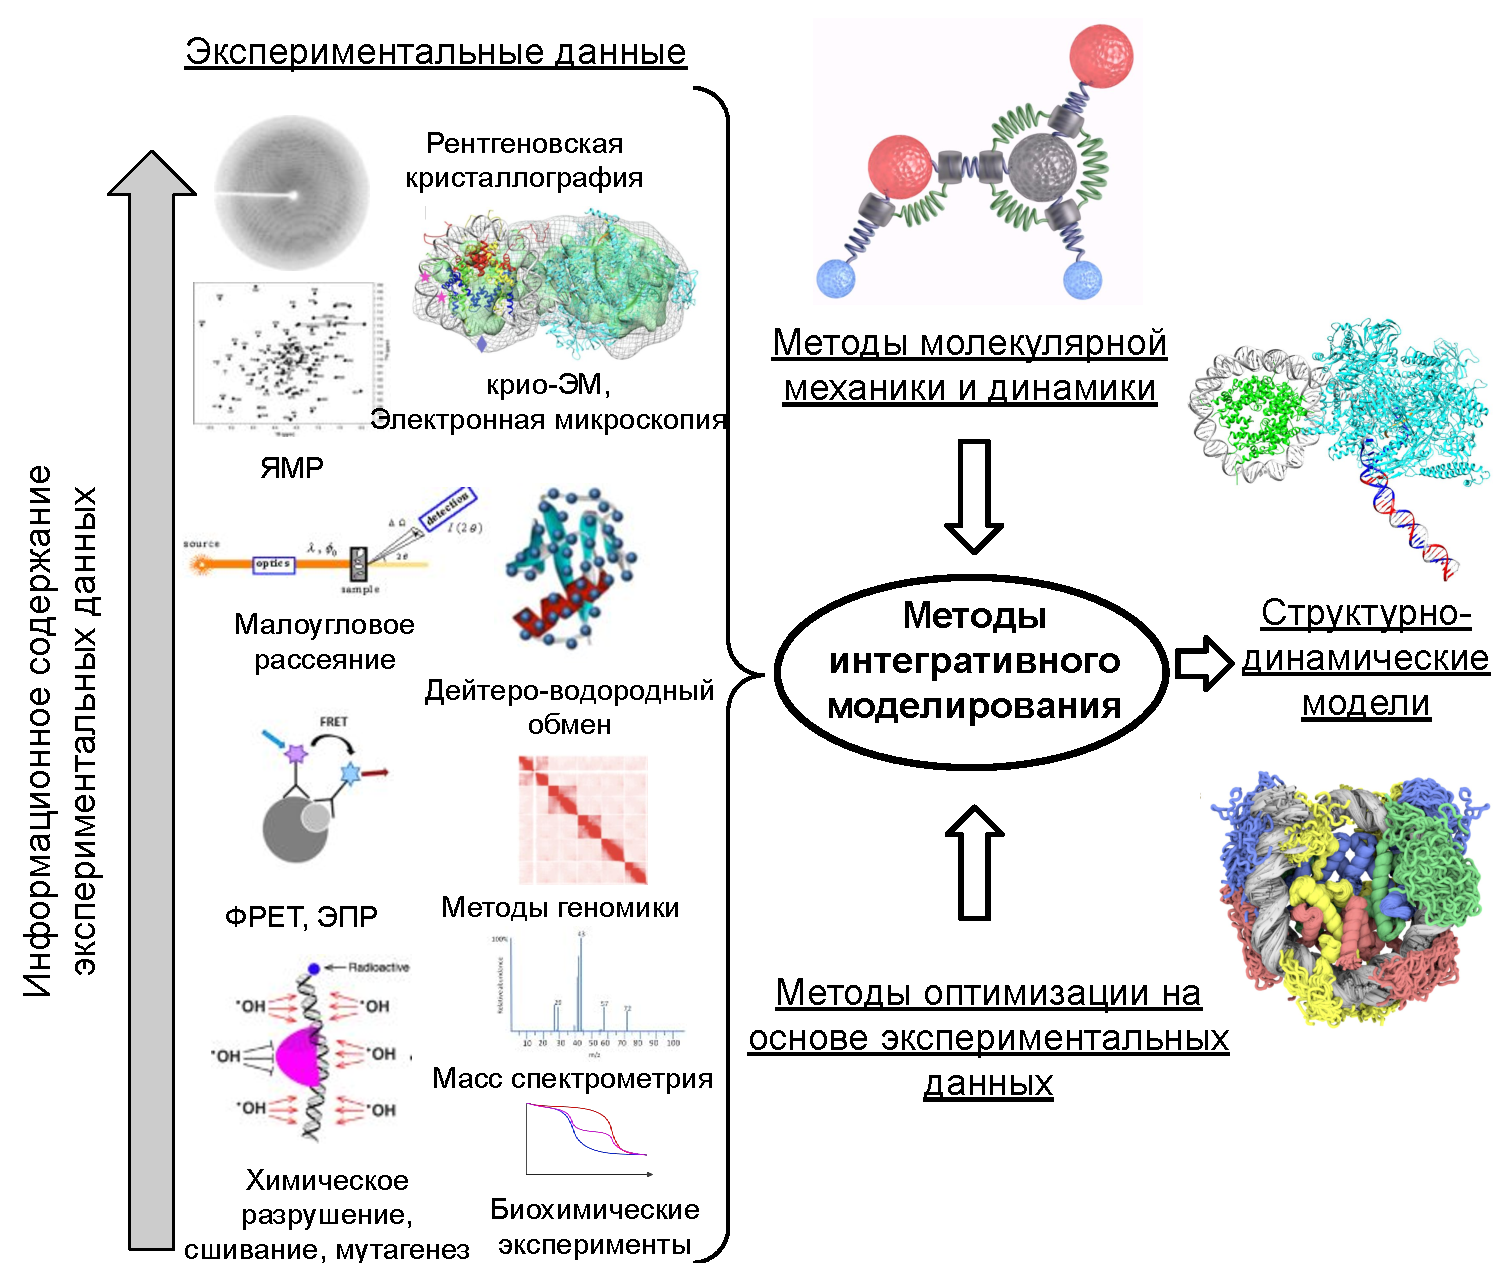
\includegraphics[height=0.9\textheight]{images/p1/int_mod.pdf}
\note{
\footnotesize{Для преодоления вышеозвученных проблем перспективным является развитие интегративных подходов к моделированию биомолекул и их комплексов.
Такие подходы предполагают интеграцию различных экспериментальных данных при построении структурно-динамических моделей биомолекул. В вычислительном плане могут применяться как возможности оптимизационного моделирования, так и имитационного моделирования на основе расчета взаимодействий между атомами.
При применении метода молекулярной динамики стандартной практикой явяляется использование экспериментально определенной стартовой конформации комплекса методами РСА, крио-ЭМ.
Для многих биологических комплексов, однако, экспериментально определенные струкутры либо отсутвуют вообще, либо неизвестны представляющие функциональные интерес конформации. В то же время часто имеются различные экспериментальные данные косвенной природы, получаемые в ходе биофизических, биохимических, функциональных, спектроскопических и других экспериментов. Такого рода эксперименты могут предоставлять информацию о расстояниях между введенными метками в белке или ДНК (например, методы FRET, ЭПР), характере укладки белковой цепи (например, ИК-, КД-спектроскопия, дифракция рентгеновских лучей на фибриллах),
реакционной доступности химических групп (методы футпринтинга, химического сшивания) и др. Задача интегративных подоходов состоит в использовании и такого рода информации.
Далее в диссертационной работе на ряде примеров будет продемонстрировано, каким образом это можно сделать. (2-11.5)}}
\end{frame}



\section[Глава 2]{Глава 2. Применение методов молекулярной динамики для изучения нуклеосом.}

\begin{frame}
\frametitle{Проблема понимания структуры хроматина}
\centering
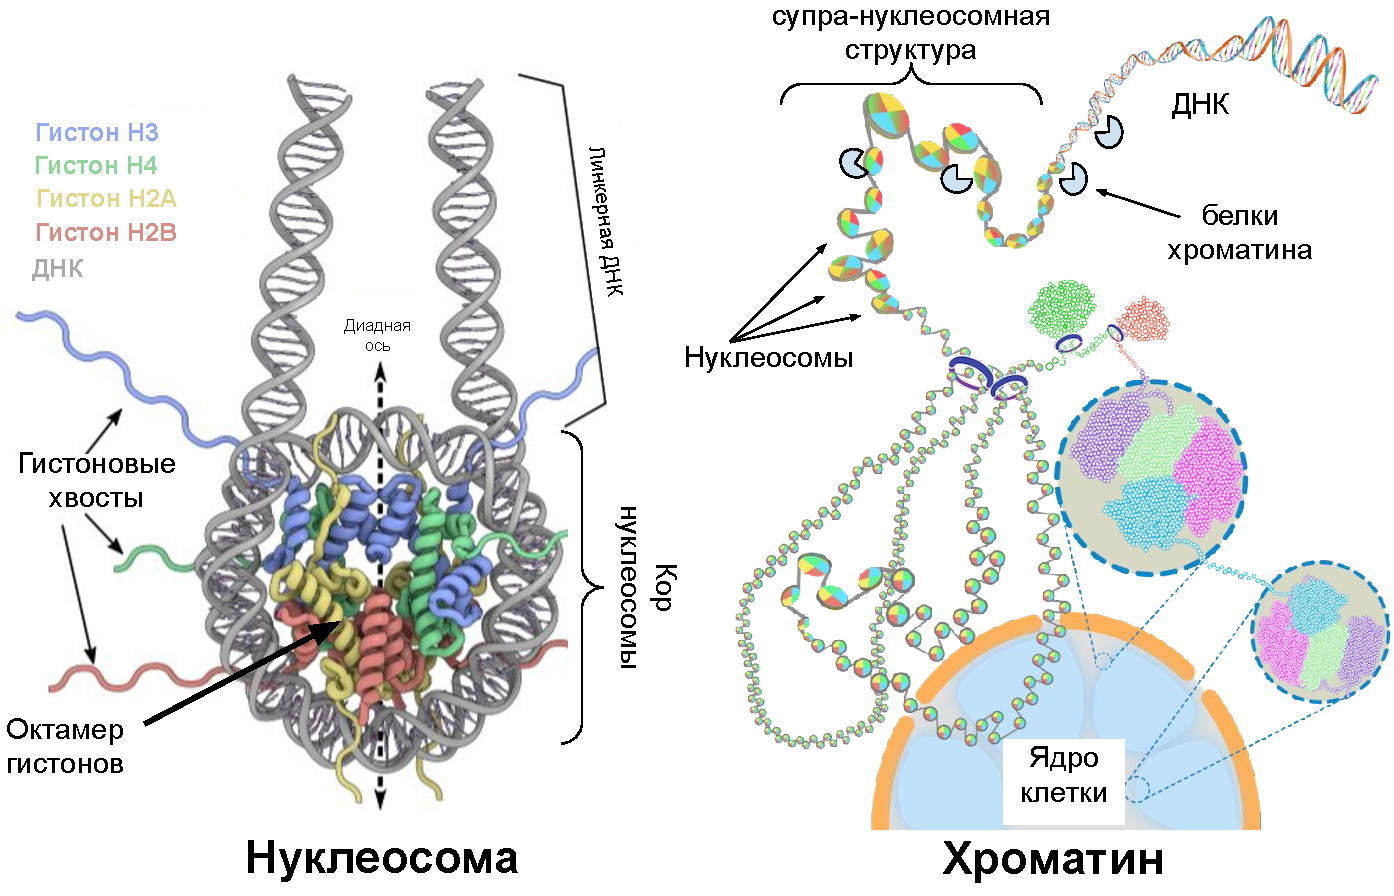
\includegraphics[width=1.0\textwidth]{s9}
\note{Первая часть работы посвящена исследованию струкутрно-динамической организации нуклеосом и их комплексов с белками хроматина. Хроматин - это набор ДНК, РНК и белков, находящихся в ядре эукариотических клеток. Нуклеосомы являются базовыми элементарными единицами хроматина. Они состоят из примерно 200 пар оснований ДНК, организованных гистоновыми белками. Центральные 147 пар оснований ДНК образуют коровую частицу нуклеосомы, плотно наматываясь на октамер гистонов в виде полутора витков левой суперспирали. Нуклеосомы претерпевают множество важных структурных и динамических перестроек во время всех ключевых процессов транскрипции, репликации, репарации ДНК и т.д. Способность нуклеосом претерпевать определенные типы конформационных переходов играет важную роль при взаимодействии с белками, включая ремоделирующие комплексы, факторы транскрипции, шапероны, РНК-полимеразы и т.д. (1.5-13)
}

\end{frame}

\begin{frame}
\frametitle{Проблема динамики нуклеосом}

\centering
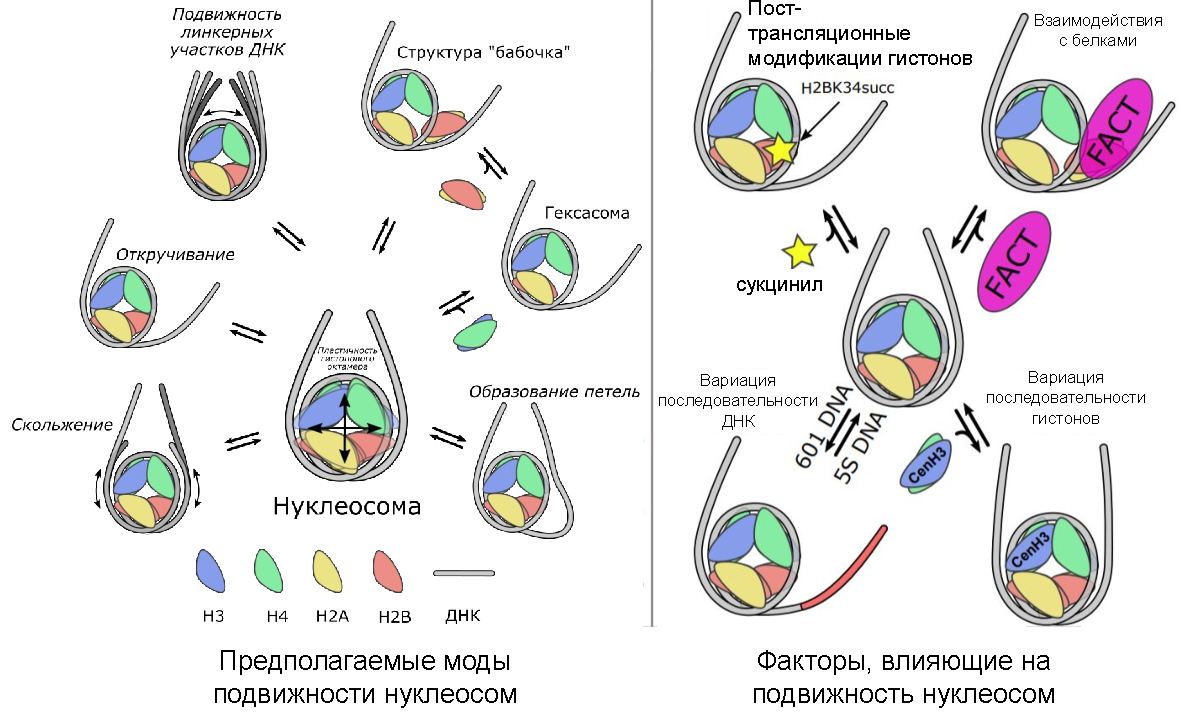
\includegraphics[width=1.0\textwidth]{s10}

\note{На слайде проиллюстрированы предполагаемые динамические режимы нуклеосом и влияние на них различных факторов:
последовательности ДНК и гистонов, пост-трансляционных модификаций аминокислот гистонов, взаимодействия с белками. Динамика нуклеосом может происходить спонтанно при данной температуре или носить функционально направленный характер за счет воздействия специальных АТФ-зависимых комплексов. Белковый состав и последовательность ДНК в нуклеосомах влияют на характер динамических процессов в нуклеосомах и таким образом модулируют различные функциональные процессы в геноме. Так показано существование тонких режимов конформационной динамики нуклеосом. Например, кручение ДНК внутри нуклеосомы обеспечивает путь для АТФ-зависимого передвижения нуклеосом вдоль ДНК. Речь идет о существовании особых режимов динамики нуклеосом, в которых важны атомостические детали структурных изменений.

В то же время, методами структурной биологии с высоким разрешением хорошо изучена лишь одна компактная конформация коровой частицы нуклеосомы, которую удалось закристаллизовать.

 Метод молекулярной динамики является мощным инструментом, который может раскрыть природу различных динамических состояний нуклеосом на атомистическом уровне. (1.5-14.5)
	
}
\end{frame}


\begin{frame}
\frametitle{Полноатомные расчеты нуклеосом методом МД}
Расчет нуклеосомы с линкерной ДНК на масштабе 1 мкс
\begin{columns}[b]
\begin{column}{0.37\textwidth}
\begin{center}
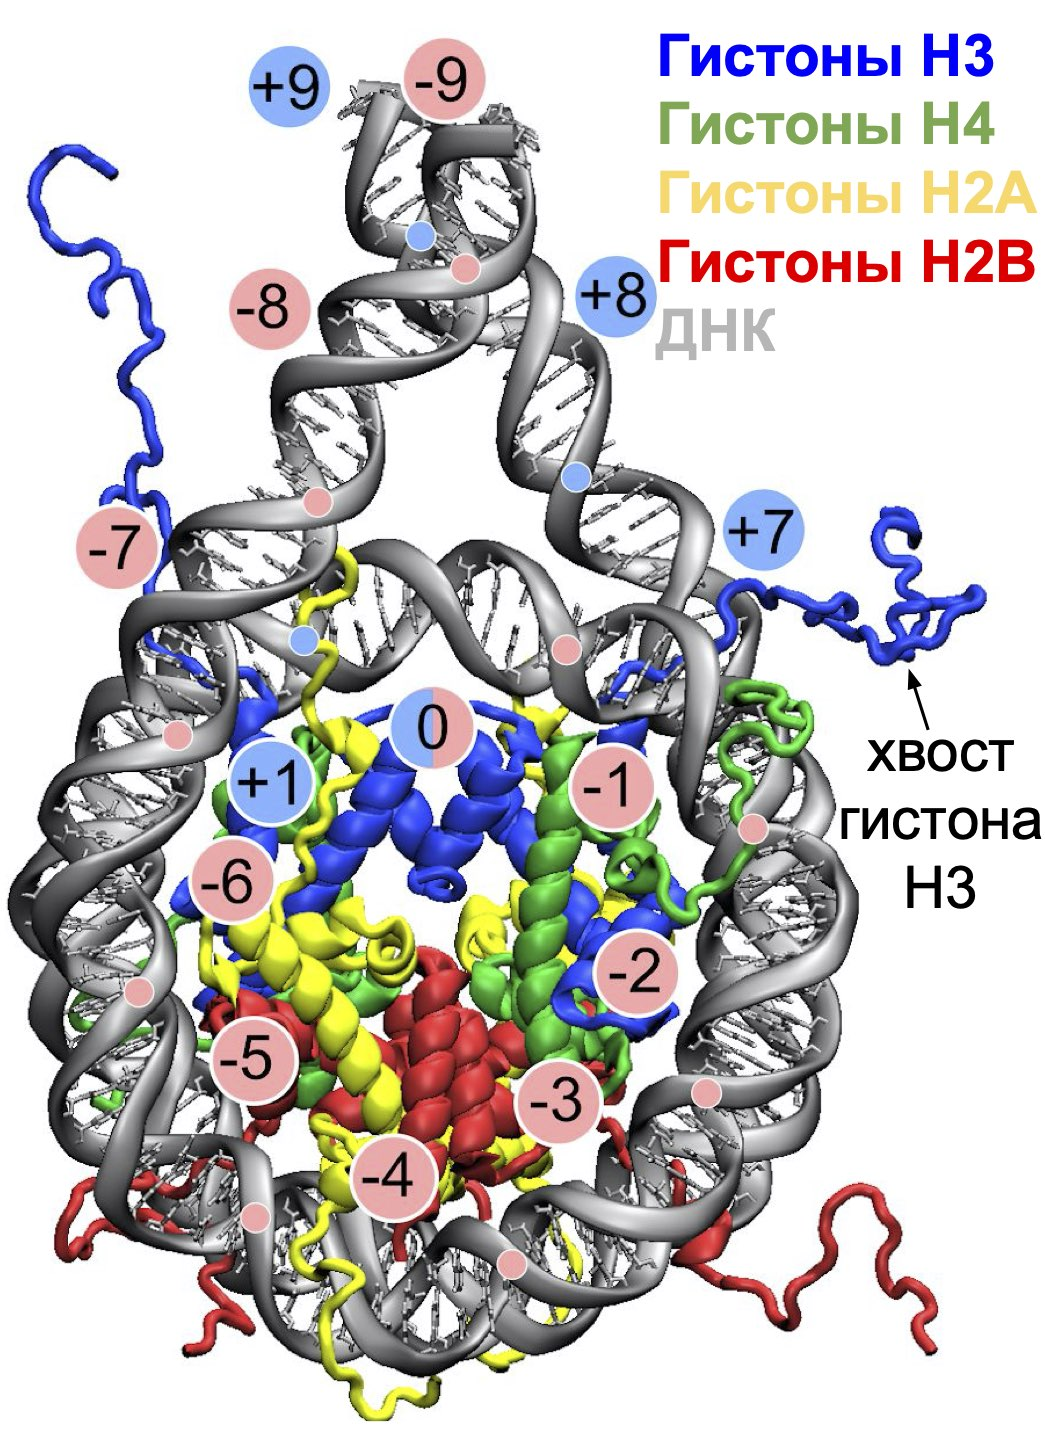
\includegraphics[width=1.0\textwidth]{s11l.jpg}
\textbf{t=0 мкс}
\end{center}
\end{column}
\begin{column}{0.32\textwidth}  %%<--- here
\begin{center}
\ifdefined\HANDOUT
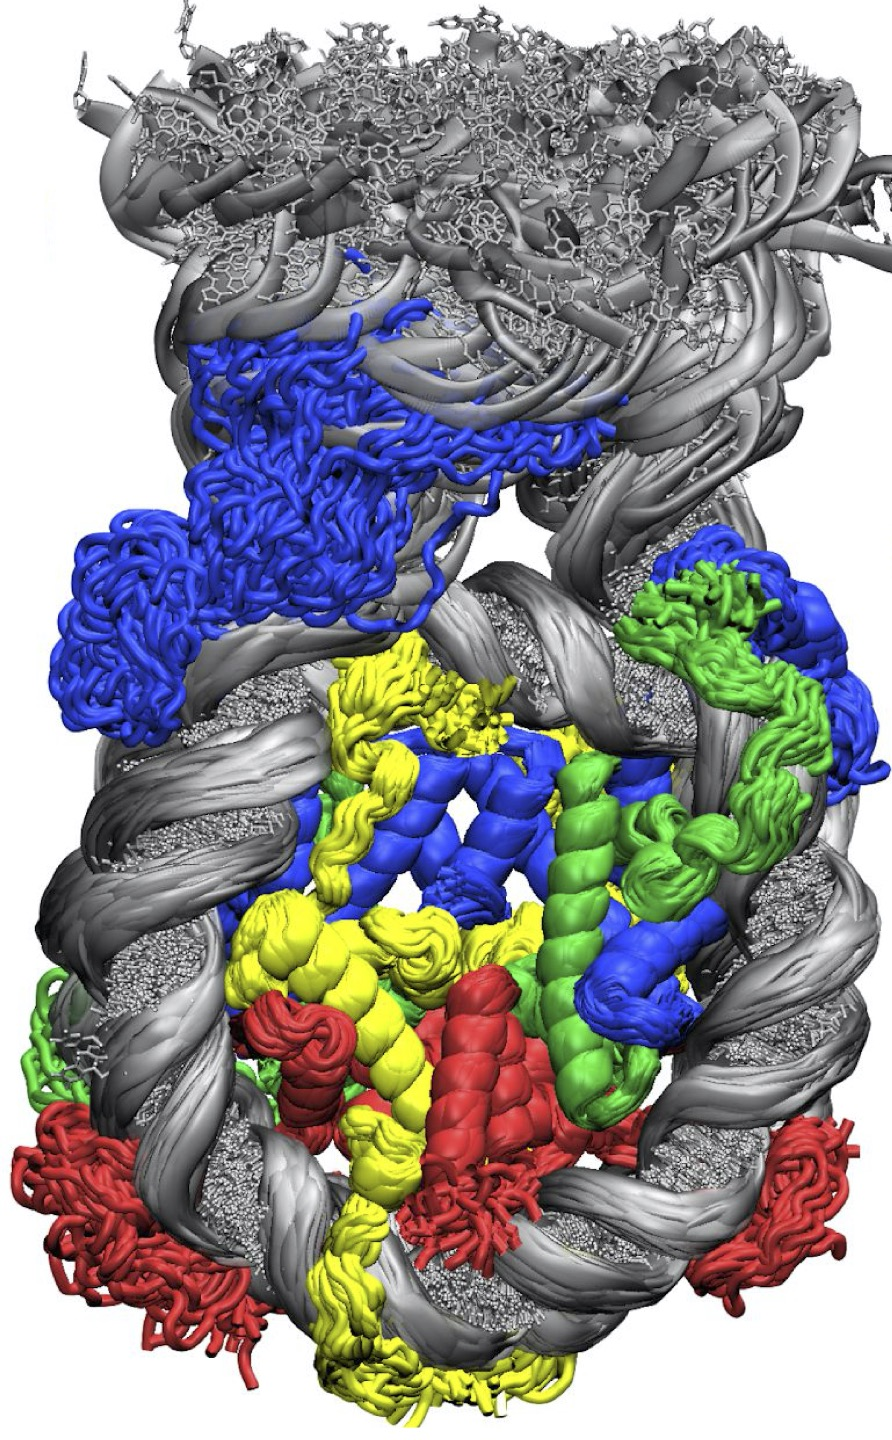
\includegraphics[width=1.0\linewidth]{1mus/1mus1}
\else
\animategraphics[width=1.0\linewidth]{10}{1mus/1mus}{1}{100}
\fi
%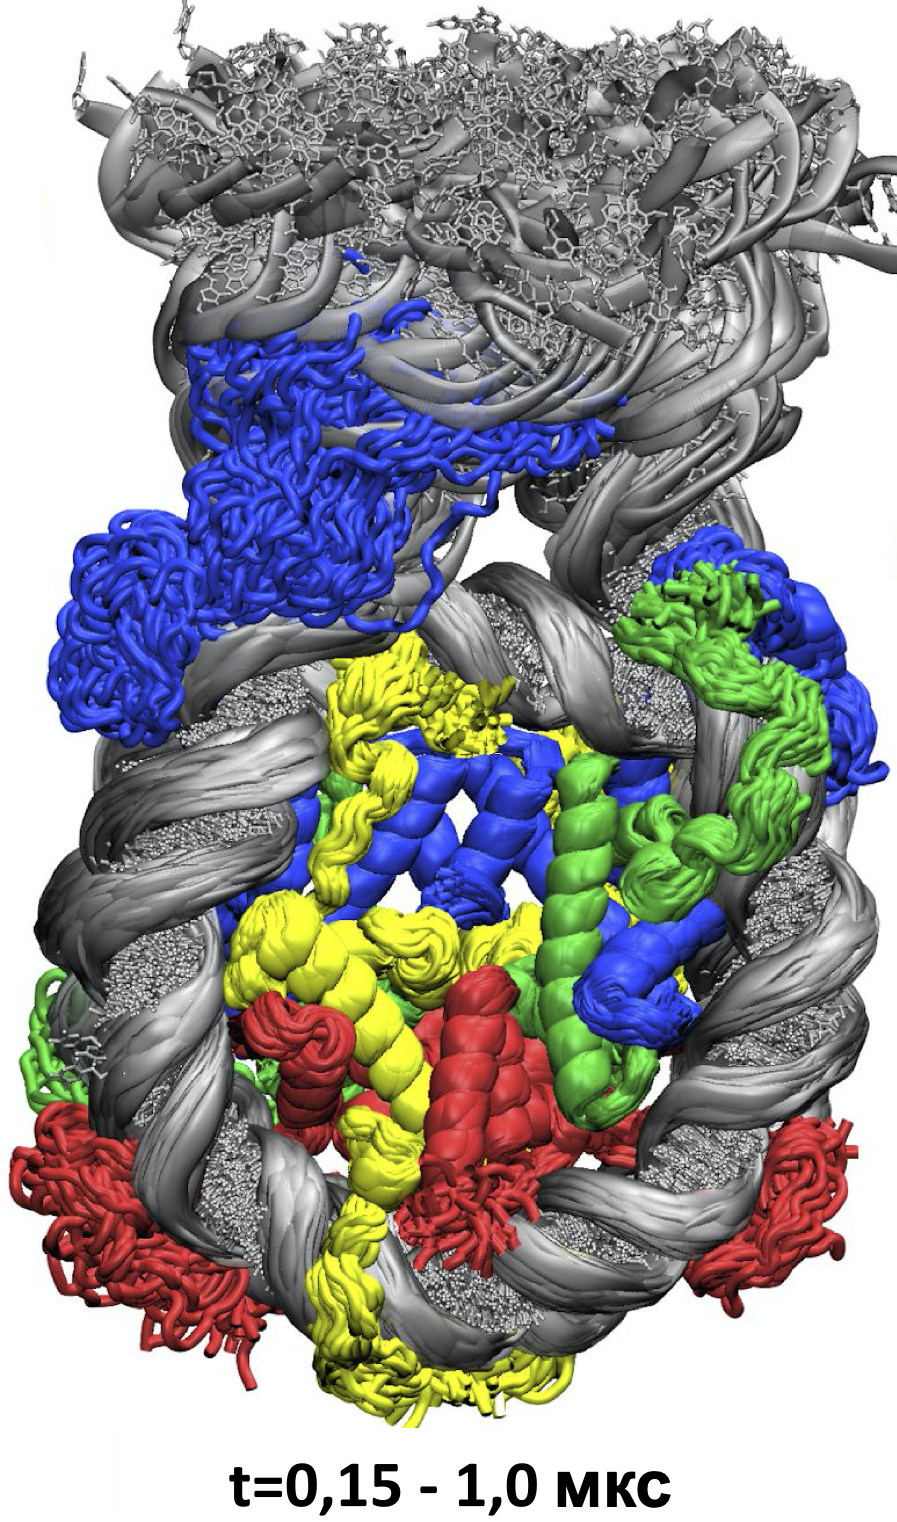
\includegraphics[width=1.0\textwidth]{s11m}
\textbf{t=0,15-1 мкс}
\end{center}
\end{column}
\begin{column}{0.31\textwidth}  %%<--- here
\begin{center}
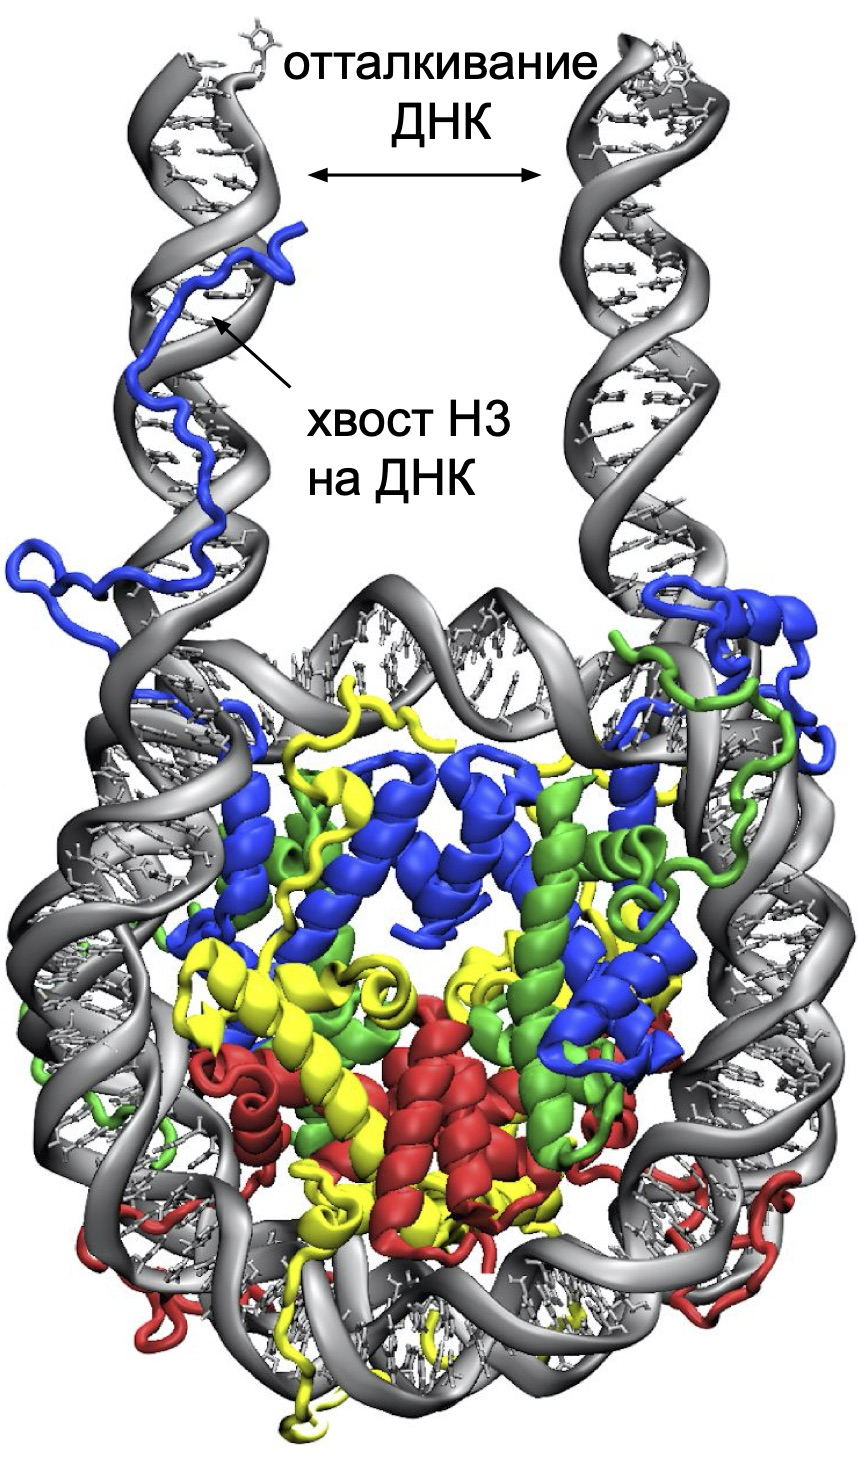
\includegraphics[width=1.0\textwidth]{s11r.jpg}
\textbf{t=1 мкс}
\end{center}
\end{column}
\end{columns}


%\centering
%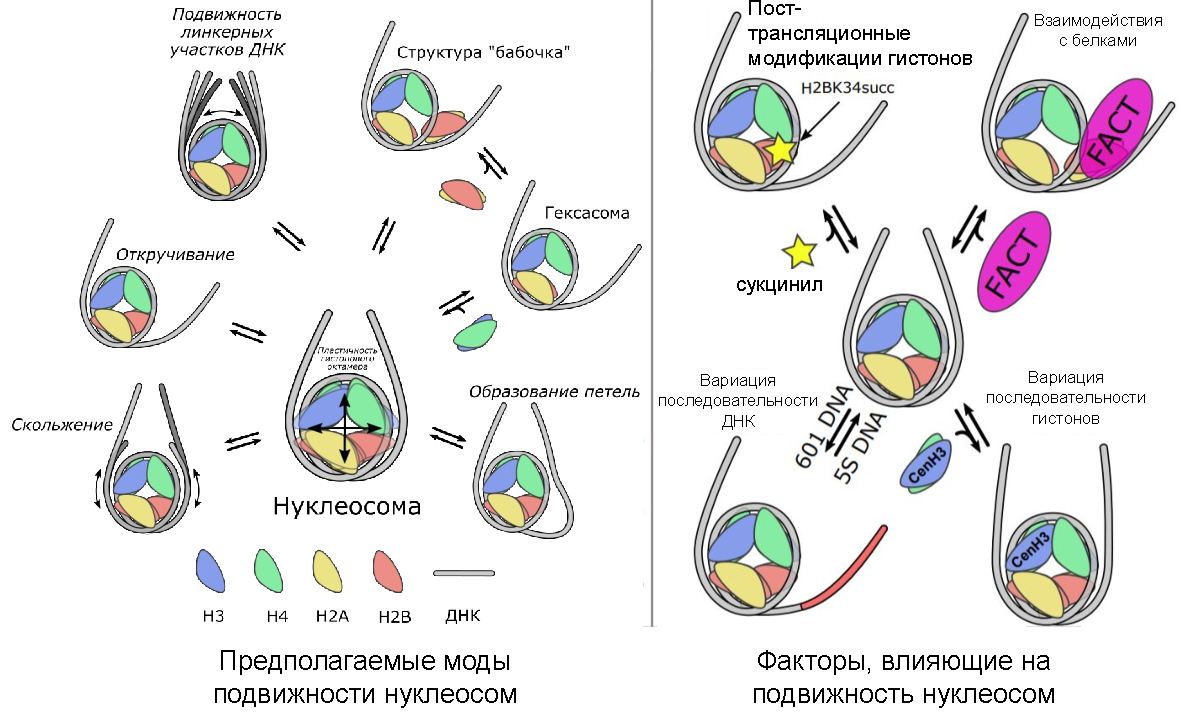
\includegraphics[width=1.0\textwidth]{s10}
% \includemedia[
%   %activate=onclick,
%   addresource=videos/nucl1mus.mp4,
%   flashvars={
%      source=videos/nucl1mus.mp4
%     &autoPlay=true
%     &loop=true
% },
%   passcontext
% ]{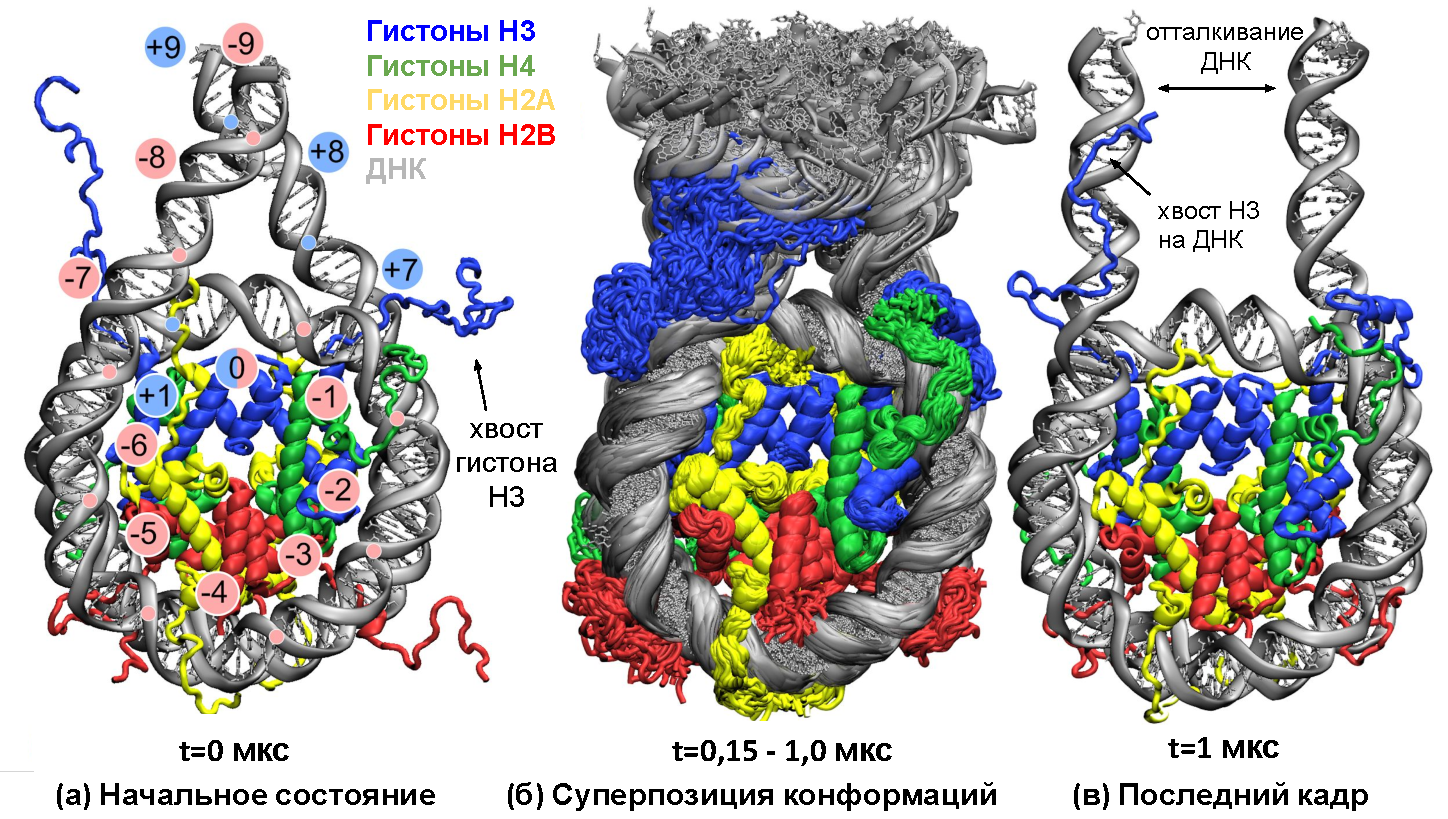
\includegraphics[height=0.45\linewidth]{images/p2/jmb/part2_2_f1}}{VPlayer9.swf}

\note{
	\tiny{Нами были разработаны подходы и алгоритмы моделирования нуклеосом методами молекулярной динамки в полноатомном приближении в явном растворителе на микросекундном и мульти-микросекундном временном диапазоне с использованием суперкомпьютерных технологий.  Также разработаны алгоритмы анализа траекторий, в частности задания нуклеосомной системы координат на основе определения оси суперспирали ДНК и оси псевдосимметрии нуклеосомы. В результате стало возможным определение различных геометрических параметров молекулярной системы таких, как геометрия ДНК, углы вращения ДНК, расположение остова полипептидных цепей. На данном слайде приводятся результаты равновесного микросекундного моделирования молекулярной динамики нуклеосом, включающих линкерные сегменты ДНК и полноразмерные гистоны. Выявлено, что линкерные участки ДНК изменяют свое взаимное расположение из-за электростатического отталкивания, что влияет на углы входа-выхода ДНК из нуклеосом и следовательно на структуру супрануклеосомной организации хроматина. Если в начальной структуре гистоновые хвосты экспонированы в растворитель, то в ходе динамики их конденсация на ДНК происходит в течение нескольких десятков наносекунд. Далее начинается диффузия хвостов вдоль поверхности ДНК. При этом хвосты могут принимать конформационно ограниченные позиции из-за вставки лизинов и аргининов в малые бороздки ДНК.
  %Мы показали, что определенные конформации гистонового хвоста способствуют выпячиванию ДНК вблизи участков ее входа/выхода в/из нуклеосомы, что приводит к образованию дефектов кручения внутри ДНК.
  Ряд аминокислот в гистоновых хвостах, являются сайтами важных эпигенетических пост-трансляционных модификаций. Видно, что многие из этих сайтов находятся в тесном контакте с ДНК, что ограничивает их доступность для пост-трансляционной модификации и взаимодействий с белками хроматина. Такие взаимодействия способствуют и возникновению кооперативных эффектов при связывании нескольких белков с соседними сайтами на гистоновых хвостах. Полученные результаты находятся в согласии с экспериментами по химическому сшиванию гистонов с ДНК, ЯМР-анализу.(2.5-17)}}
\end{frame}


\begin{frame}
\frametitle{Мульти-микросекундные МД расчеты нуклеосом}
%\embedvideo{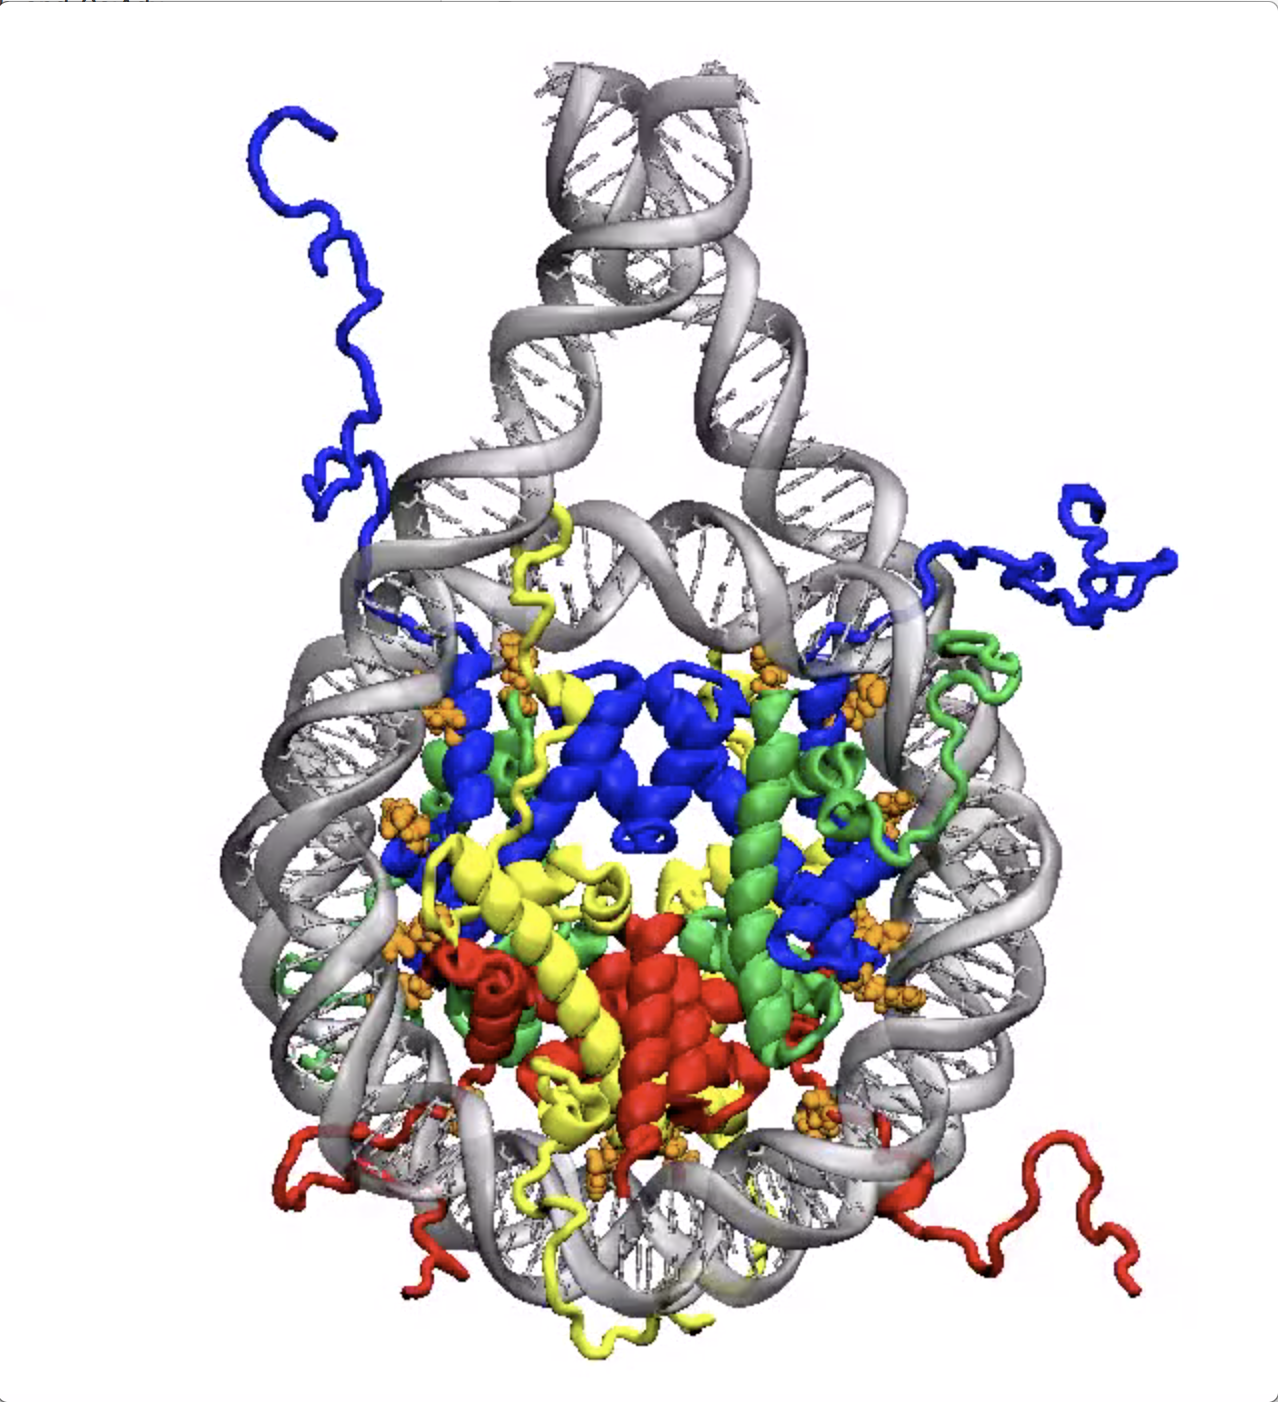
\includegraphics[width=0.45\textwidth]{Presentation/images/nucl1mus}}{videos/nucl1mus.mp4}

Расчет коровой частицы нуклеосомы на масштабе > 10 мкс
\begin{columns}[b]
\begin{column}{0.3\textwidth}
\begin{center}
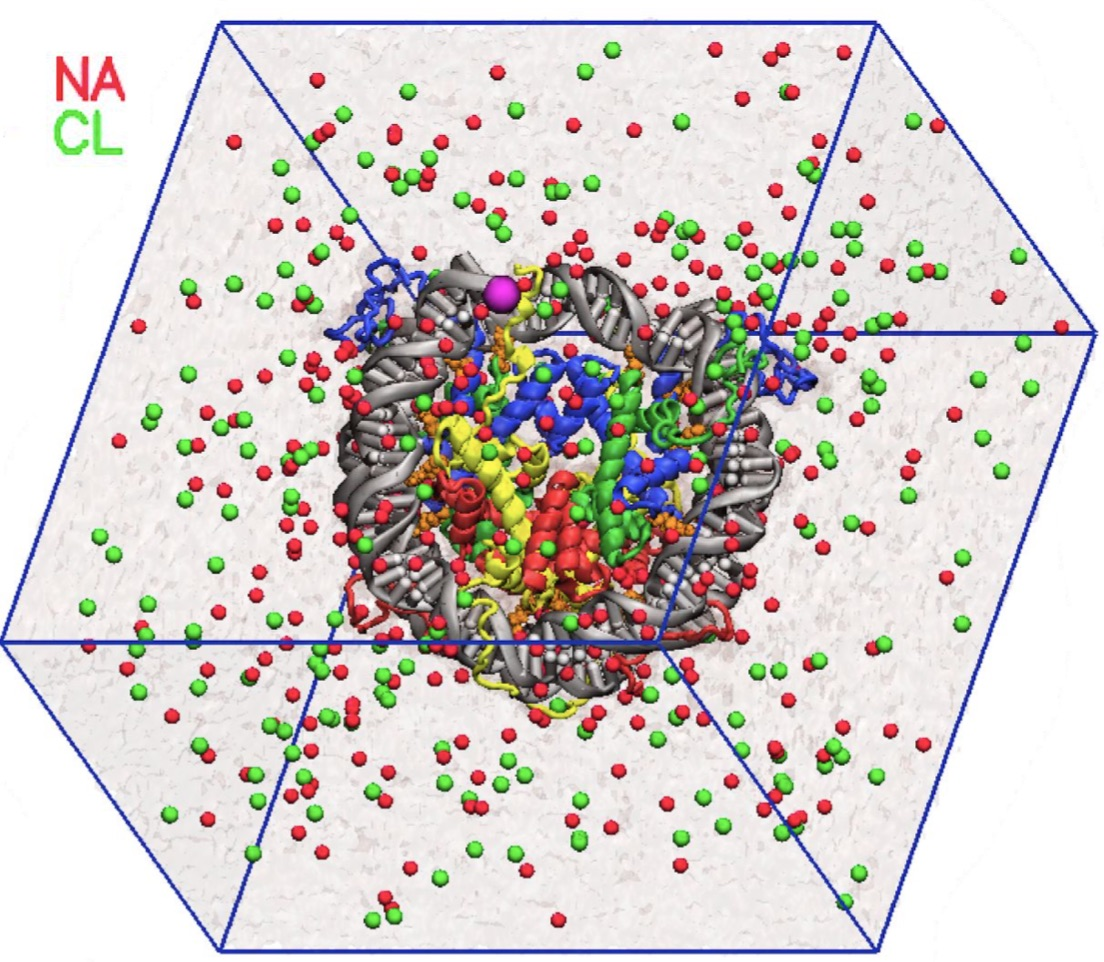
\includegraphics[width=1.0\textwidth]{s12l.jpg}
Расчетная система в растворителе
\end{center}
\end{column}
\begin{column}{0.45\textwidth}  %%<--- here
\begin{center}
% \animategraphics[width=1.0\linewidth]{10}{10mus/10mus}{1}{100}
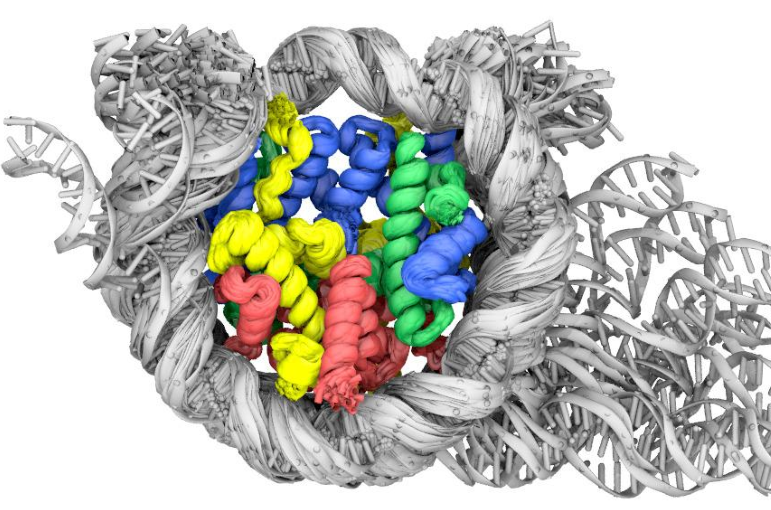
\includegraphics[width=1.0\textwidth]{s12m}
Динамика системы
\end{center}
\end{column}
\begin{column}{0.25\textwidth}  %%<--- here
\begin{center}
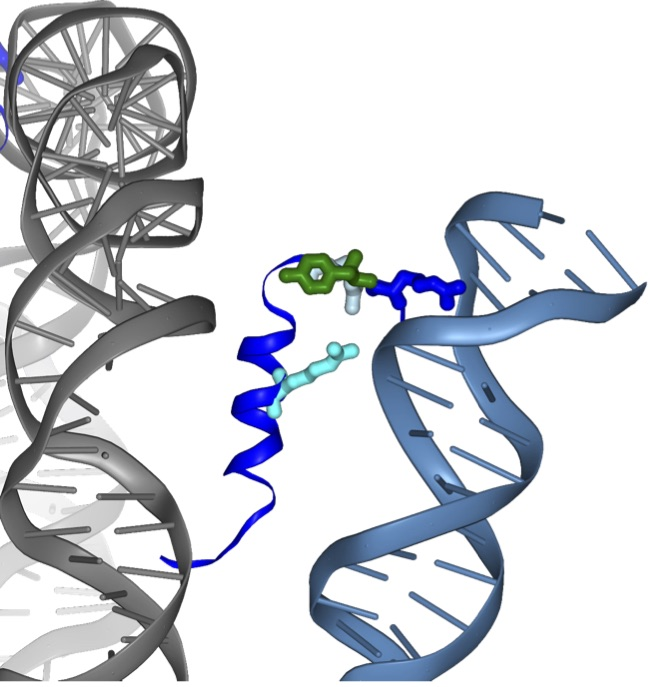
\includegraphics[width=1.0\textwidth]{s12r.jpg}
Динамика гистонов влияет на откручивание ДНК
\end{center}
\end{column}
\end{columns}

\note{\scriptsize{На данном слайде представлено развитие предыдущей работы - моделирование коровых частиц нуклеосом на временах более 10 мкс, которое стало возможным и благодаря прогрессу вычислительных технологий и разработанной нами автоматической системе подготовки, запуска и анализа расчетов. На столь длинных временах мы впервые наблюдали диссоциацию и откручивание ДНК от гистонового октамера. В ходе моделирования были выявлены ключевые взаимодействия ДНК-белок с гистонами, которые являются барьерами для откручивания ДНК от октамера гистонов. На рисунке показана такая область белка вблизи конца нуклеосомной ДНК. Механизм сцепления двух супервитков ДНК заключается в том, что боковые цепи соседних аминокислот взаимодейстуют с малыми бороздками. Потеря одного из контактов приводит к возникновению флуктуаций ДНК. В ходе моделирования также была показана возможность локального спонтанного изменения степени закрученности ДНК (образование/релаксация так называемых дефектов кручения) и сдвиг ориентационного положения для части коровой ДНК. Данные наблюдения указывают на возможность транслокации ДНК вдоль нуклеосомы путем “червячного” передвижения дефектов кручения вдоль ДНК (inchworm meсhanism). При этом ДНК подобно винту прокручивается вдоль поверхности октамера гистонов. В ходе моделирования также было показано наличие динамической пластичности ядра гистонов, способствующей подвижности ДНК. В результате сравнительного моделирования нуклеосом с хвостами и без хвостов гистонов было выявлено, что гистоновые хвосты замедляют как время отворачивания, так и время приворачивания ДНК, а также при отворачивании ДНК удерживают ее вблизи исходной траектории. (2.5-19.5)}}
\end{frame}

\section[Глава 3]{Глава 3. Интегративное моделирование с применением данных экспериментов по футпринтингу ДНК.}


\begin{frame}
\frametitle{Метод гидроксильного футпринтинга}

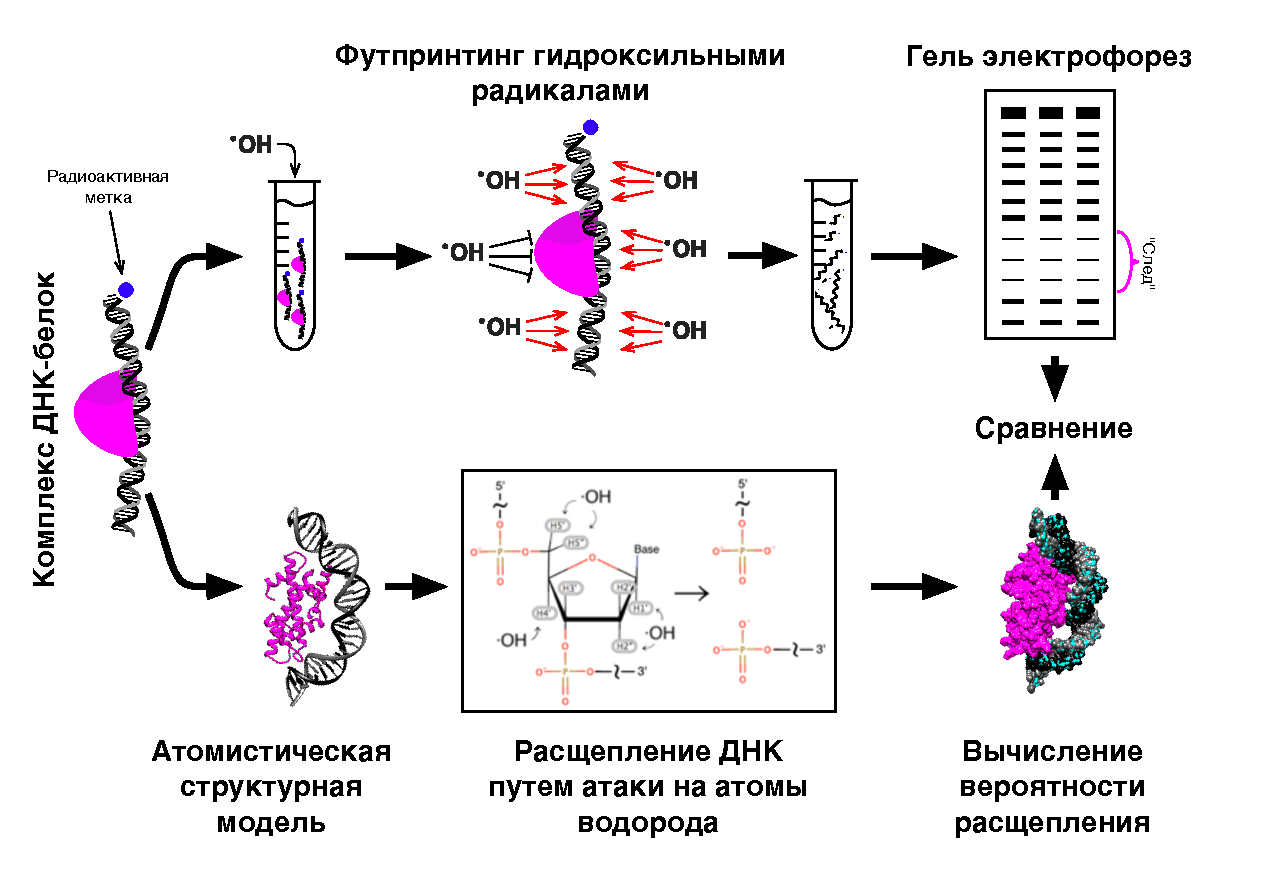
\includegraphics[width=1.0\textwidth]{images/p5/part5_1_np/p5_1_f1.pdf}

\note{Процессы динамики нуклеосом, изученные нами методом МД, ограничены по времени в силу текущих вычислительных возможностей. Крупномасштабные процессы, например, скольжения нуклеосом вдоль ДНК, сборка и разборка нуклеосом, полная диссоциации/реассоциации ДНК пока находятся за пределами моделируемых временных интервалов. Примером задачи не решаемой методами МД является выбор нуклеосомой наиболее энергетически выгодного оптимального положения на большом участке ДНК. Для решения такой задачи могут применяться интегративные подходы. В главе 3 развиты подходы по моделированию ДНК-белковых комплексов, основанные на использовании экспериментальных данных по расщеплению ДНК (футпринтингу) гидроксильными радикалами. Гидроксильные радикалы обладают высокой реакционной способностью, небольшим размером, не являются заряженными. При взаимодействии с ДНК они атакуют атомы водорода дезоксирибозы, что приводит к расщеплению ДНК с потерей атакованного нуклеотида. При наличии белка на ДНК, белок стерически экранирует ДНК от расщепления. Это свойство можно использовать для анализа структуры ДНК-белковых комплексов. Общая схема данного подхода представлена на слайде.(1.5-21)}
\end{frame}


\begin{frame}
\frametitle{Проблема интерпретации данных футпринтинга ДНК}
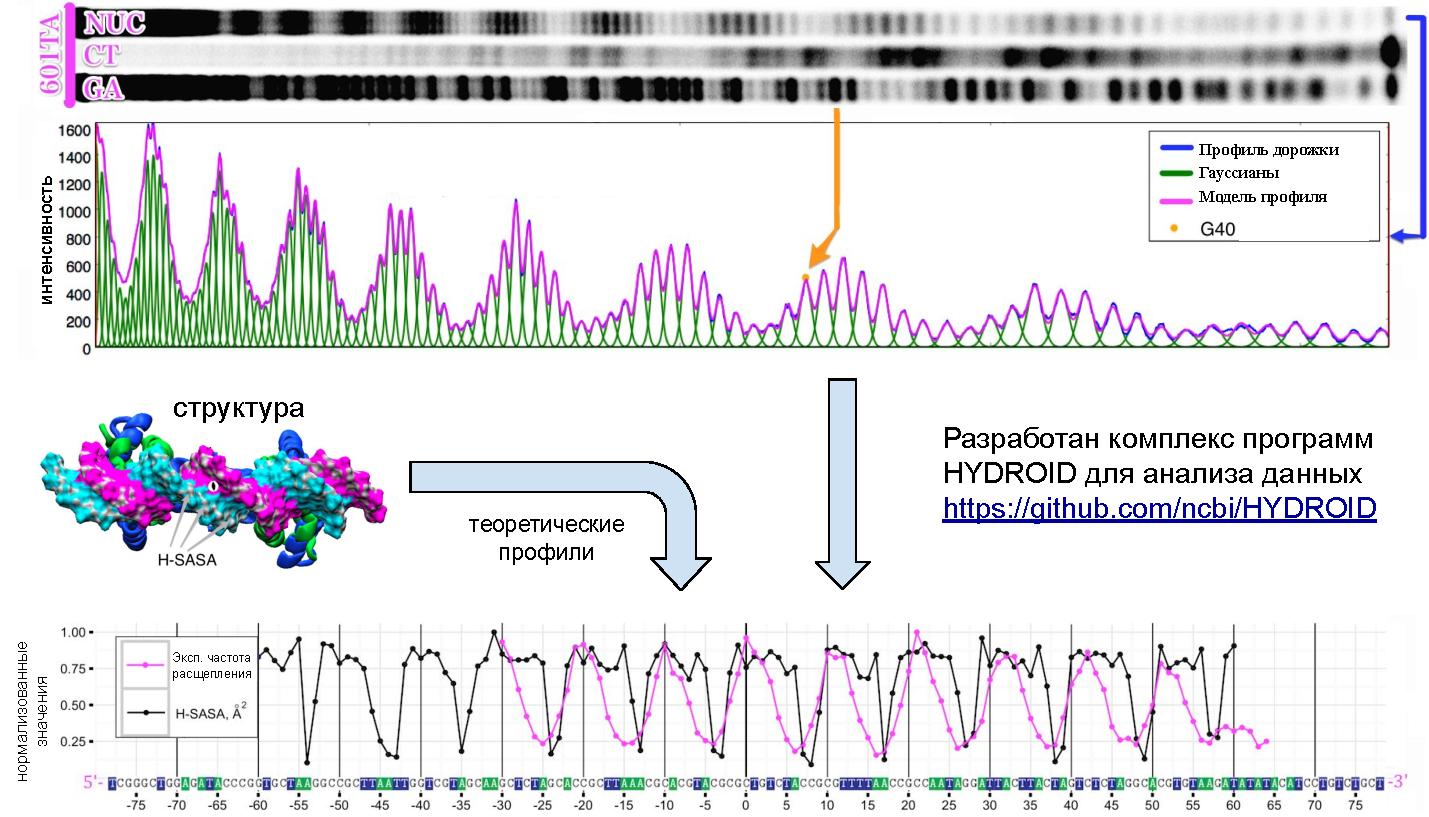
\includegraphics[width=1.0\textwidth]{s14}

\note{В методе гидроксильного футпринтинга фрагменты расщепленных молекул ДНК визуализируют с помощью метода гель-электрофореза. Гель электрофорез разделяет молекулы по длине и формируется характерная картина полос разной интенсивноси. При этом суммарная интенсивность полосы пропорциональна вероятности расщепления ДНК в конкрентной позиции. У каждой полосы присутствует диффузионное размытие, зависящее от длины фрагмента ДНК. Определение интенсивности полос требует аппрокисмации данных в виде математической модели (каждая полоса описывается гауссом). Нами был разработан программный продукт HYDROID позволяющий вычислять профили интенсивонсти расщепления ДНК по изображениям гель электрофореза, а с другой стороны оценивать эту величину на основе моделей ДНК-белковых комплексов. Для оценки был разработан алгоритм, который оценивает доступность атомов водорода деоксирибозы для атаки гидроксильными радикалами.(1.5-22.5)}
\end{frame}


\begin{frame}
\frametitle{Определение позиционирования ДНК на нуклеосоме}
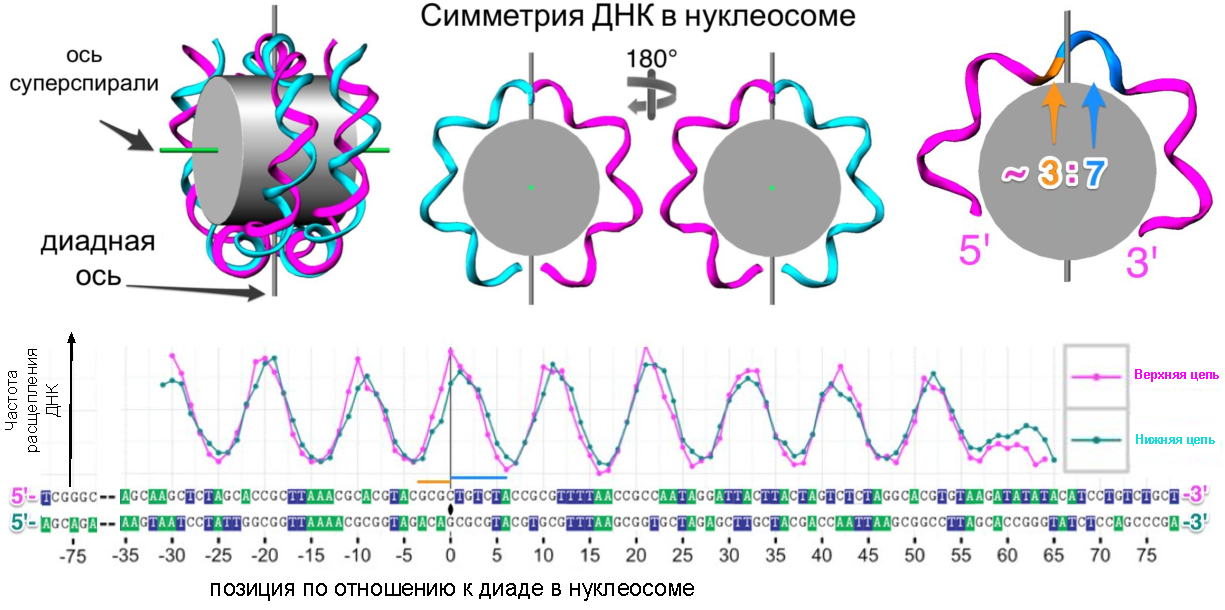
\includegraphics[width=1.0\textwidth]{s15}
\note{Используя разарботанные подоходы по обработке экспериментальных данных гидроксильного футпринтинга, а также теоретического моделирования этого процесса на основе структурных моделей, нами был разработан алгоритм, который позволяют точным образом определить положение ДНК в нуклеосоме. Дело в том, что в зависимости от характеристик ДНК сиквенса стабильность нуклеосомы может отличаться на 2-4 ккал/моль. Таким образом, на длинном фрагменте ДНК белковое ядро соберется в определенной выгодной конфигурации. Оказывается, что определить эту конфигурацию можно по данным футпринтинга с точность до одного нуклеотида, если учесть свойства симметрии нуклеосомы. Поскольку нуклеосома обладает осью псевдо симметрии второго порядка, то при повороте на 180 градусов одна цепь ДНК занимает положение другой. Это проявляется и в совпадении профилей футпринтинга для двух цепей ДНК, если они выровнены по нулеотидоной паре, лежащей на оси симметрии - диаде. А если эта пара не известна, то ее можно установить решив обратную задачу и таким образом опеределить положение ДНК на белковом ядре. (1.5-24)}
\end{frame}


\begin{frame}
\frametitle{Реконструкция неизвестной структуры нуклеосомы}
\begin{columns}[t]
\begin{column}{0.4\textwidth}
\begin{center}
\ifdefined\HANDOUT
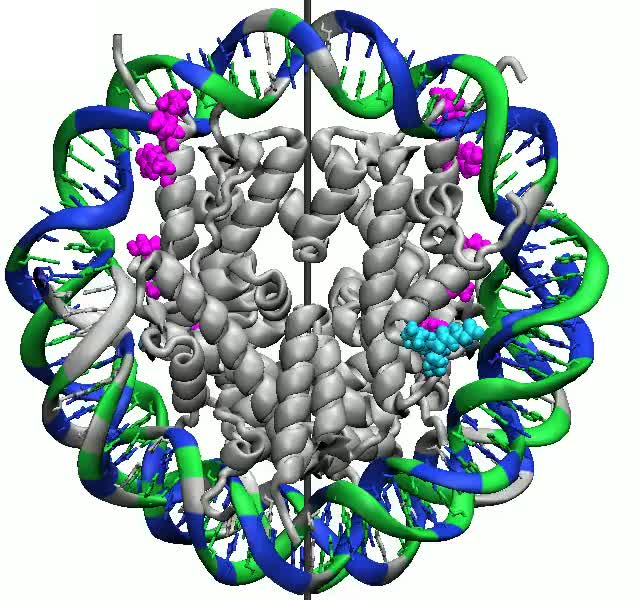
\includegraphics[width=1.0\linewidth]{cennuc/cennuc1}
\else
\animategraphics[autoplay,loop,width=1.0\linewidth,every=2]{10}{cennuc/cennuc}{1}{359}
\fi
\end{center}
\end{column}
\begin{column}{0.6\textwidth}  %%<--- here
\begin{center}
% \animategraphics[width=1.0\linewidth]{10}{10mus/10mus}{1}{100}

Задача: реконструкция структуры центромерной нуклеосомы пекарских дрожжей \textit{S. cerevisiae}.
\begin{itemize}
  \item На рисунке модель нуклеосомы третьей хромосомы дрожжей.
  \item Необычный сиквенс ДНК с А-траками функционально важен.
\end{itemize}
\end{center}
\end{column}
\end{columns}
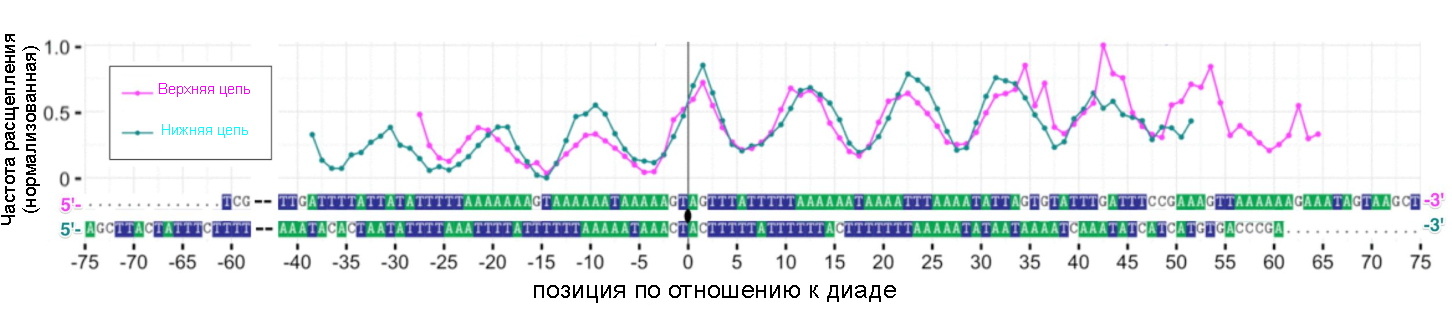
\includegraphics[width=1.0\textwidth]{s16b}
\note{Такой метод был использован нами, чтобы на основе известных структур нулеосомы и данных гидроксильного футпринтинга построить модель одной из центромерных нуклеосом пекарских дрожжей. После того, как определено положение ДНК, метод построения аналогичен методу построения моделей белков по гомологии. Точное позиционирование ДНК в модели важно для установления структуры поверхности, которая узнается белками кинетохоры. ДНК на нуклеосоме подобно винту (червячной передаче) трансляционное смещение на 1 нуклеотид сопряжено с ротационым поворотом на 36 градусов, что меняет конфигурацию поверхности узнаваемой белками. Известно, что для работы центромерных нуклеосом важны как особенности поверхности белка, так и сиквенс ДНК. (1-25)}
\end{frame}

\section[Глава 4]{Глава 4. Моделирование комплексов нуклеосом с белками хроматина.}

\begin{frame}
\frametitle{Проблема понимания супрануклеосомных структур}
\begin{columns}[t]
\begin{column}{0.5\textwidth}
\begin{center}
\underline{Огрубенное представление}
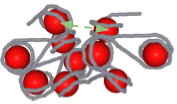
\includegraphics[width=1.0\textwidth]{s17l}
Хроматин в представлении бусин на нити. Красные шары - октамеры гистонов, синяя нить - ДНК.
\end{center}
\end{column}
\begin{column}{0.5\textwidth}  %%<--- here
\underline{Атомистическое представление}
\begin{center}
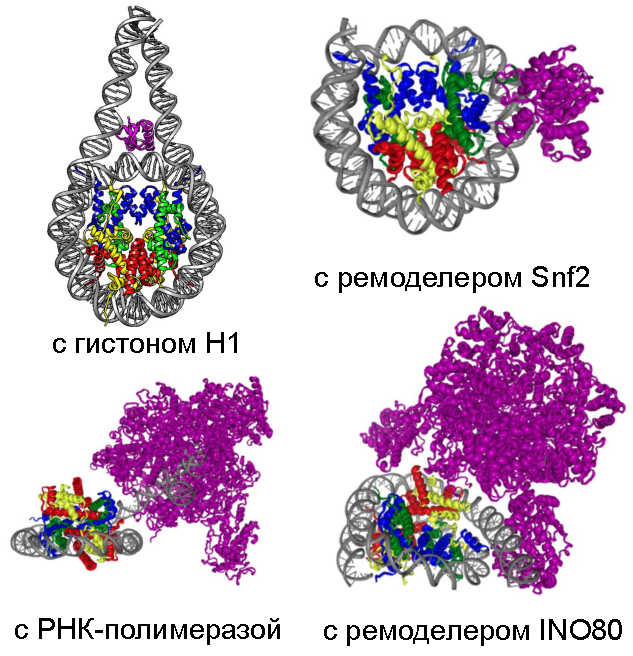
\includegraphics[width=1.0\textwidth]{s17r}
 % \begin{itemize}
 %        \item Ограниченные времена моделирования
 %        \item Времена функциональной динамики комплексов существенно больше
 %        \item Ограниченная точность силовых полей
 %        \item Чувствительность конформаций комплексов к точности параметров моделирования
 %    \end{itemize}
\end{center}
\end{column}
\end{columns}
\note{Следующая глава как раз посвящена изучению наднуклеосомной структуры. Это та инетересная область, где встречаются структурная биология и полимерная физика. С одной стороны возможно огрубленное описание как на рисунке слева. Данная модель построена путем огрубления случайных конформаций нуклеосом, полученных нами в МД, и их соединения прямыми участками ДНК. С другой стороны в хроматине присутвует большое количество белков взаимодействующих определенным образом с нуклеосомами и здесь необходимо учитывать и атомистическое представление. Из-за большого размера таких систем применение методов МД к ним затруднительно, однако можно применять различные интегративные и огрубленные подходы. (1-26)}
\end{frame}

\begin{frame}
\frametitle{Комплексы нуклеосом и РНК-полимераз}
\centering
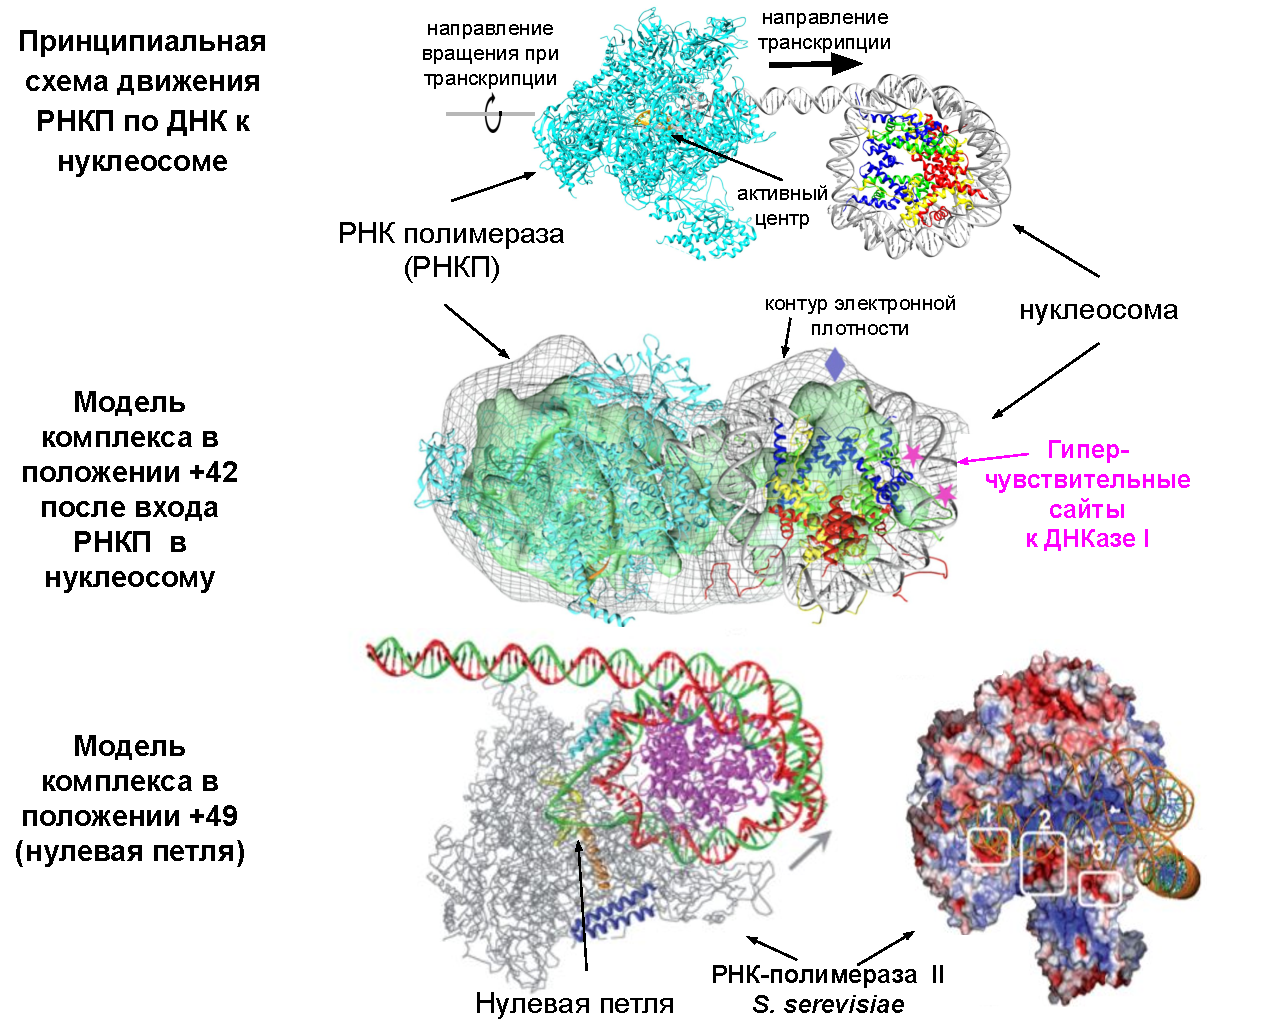
\includegraphics[height=0.9\textheight]{s18}
\note{На слайде представлен пример проведенного нами моделировния комплексов РНК полимеразы с нуклеосомой. РНК полимераза осуществляет считывание кода последовательности ДНК и синетз РНК. При этом она распрлетает ДНК и следует винтовой траектории ДНК. Возможность прохождения РНК вокруг нуклеосомы без ее разборки важно для сохранения эпигенетических меток. Здесь представлены модели структур нуклеосомы, когда ее активный сайт находится в $+42$ и $+49$ положении после входа в нуклеосому, построеные по данным футпринтинга и электронной микроскопии. Характерной особенность комплекса $+49$ ``нулевой петли'' является формирование полтного взаимодействия ДНК с гистонами как до, так и после полимеразы. Анализ электростатического потенциала указывает на то, что стабильности данного комплекса способствует наличие отрицательно заряженных остатков в местах контактов с положительно заряженными гистонами.(1.5-27.5)}
\end{frame}

\begin{frame}
\frametitle{Использование данных FRET}

\begin{columns}[t]
\begin{column}{0.5\textwidth}
\centering
Эффект Ферстеровского резонансного переноса энергии\\
\medskip
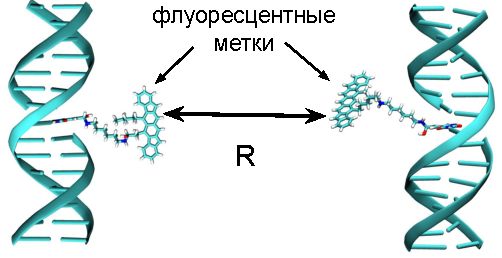
\includegraphics[width=1.0\textwidth]{s19l}

Эффективность переноса энергии с донора на акцептор

    $$E_{FRET}=\frac{1}{1+(R/R_0)^6}$$
    $R_0$ - радиус Ферстера
\end{column}
\begin{column}{0.5\textwidth}  %%<--- here



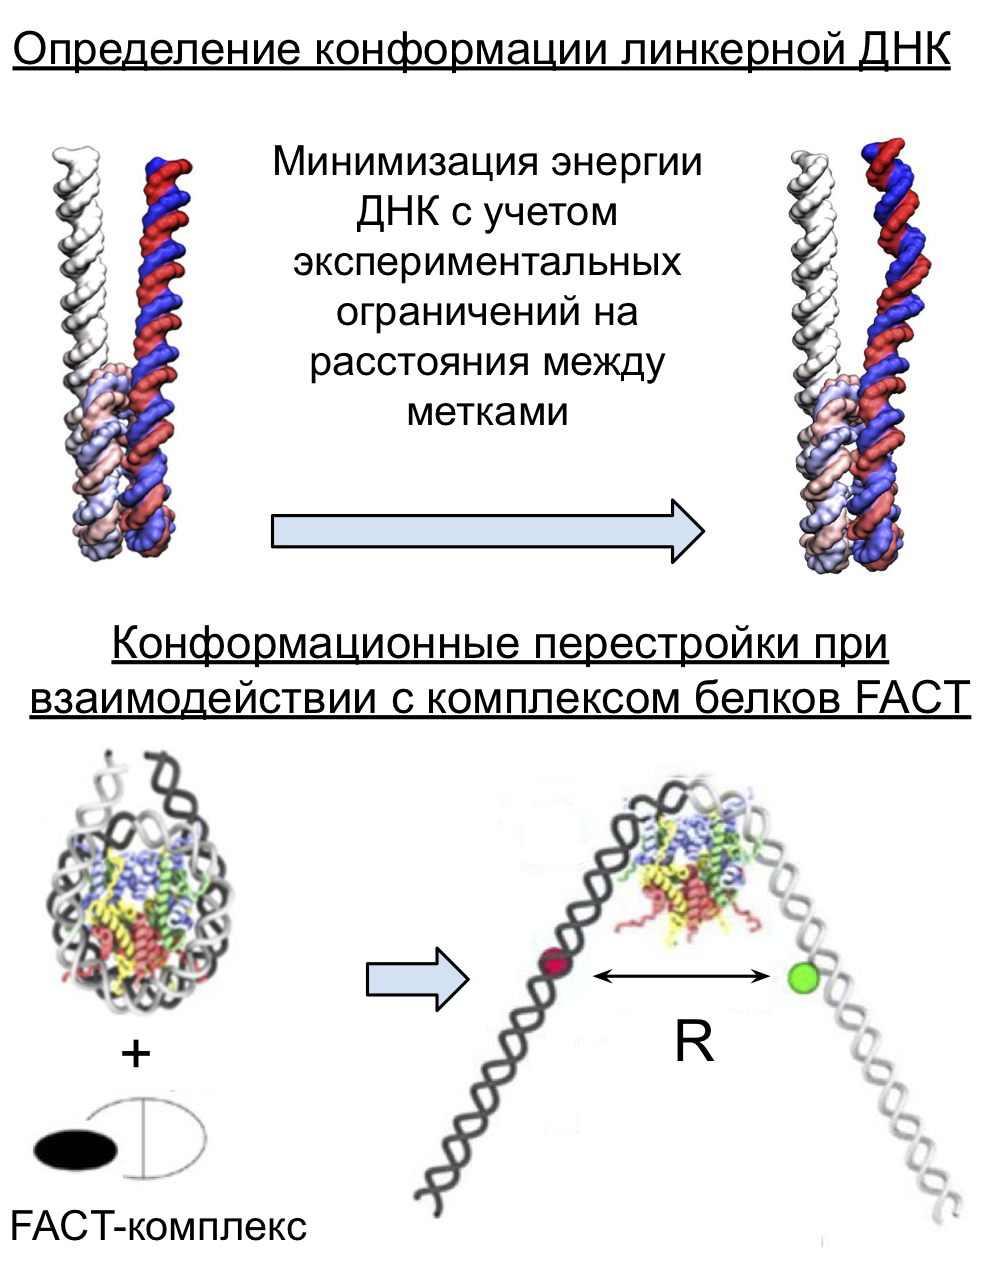
\includegraphics[width=1.0\textwidth]{s19r}
% \animategraphics[width=1.0\linewidth]{10}{10mus/10mus}{1}{100}

\end{column}
\end{columns}

\note{Еще одним видом данных, которые можно использовать для интегративного моделирования, являются данные экспериментов ФРЕТ. Эффект ФРЕТ возникает между двумя флуорестцентными метками, находящимися рядом с перектывающимися спектрами излучения и поглощения и заключается в безызлучательном переносе возбуждения с метки донора на метку акцептора. Регистрируя интенсивность данного эффекта спектроскопическими методами можно делать выводы о расстояниях между метками. Данные расстояния можно использовать для оптимизации и отбора огрубленных моделей молекулярных систем, соответствующих эксперименатльным данным. В работе нами такой подход использовался для построения моделей линкерных участков ДНК в нуклеосомах, а также для построения моделей разворачивания нуклеосом при из взаимодействии с комплексом белков FACT.(1-28.5)}
\end{frame}

\begin{frame}
\frametitle{Использование данных футпринтинга}
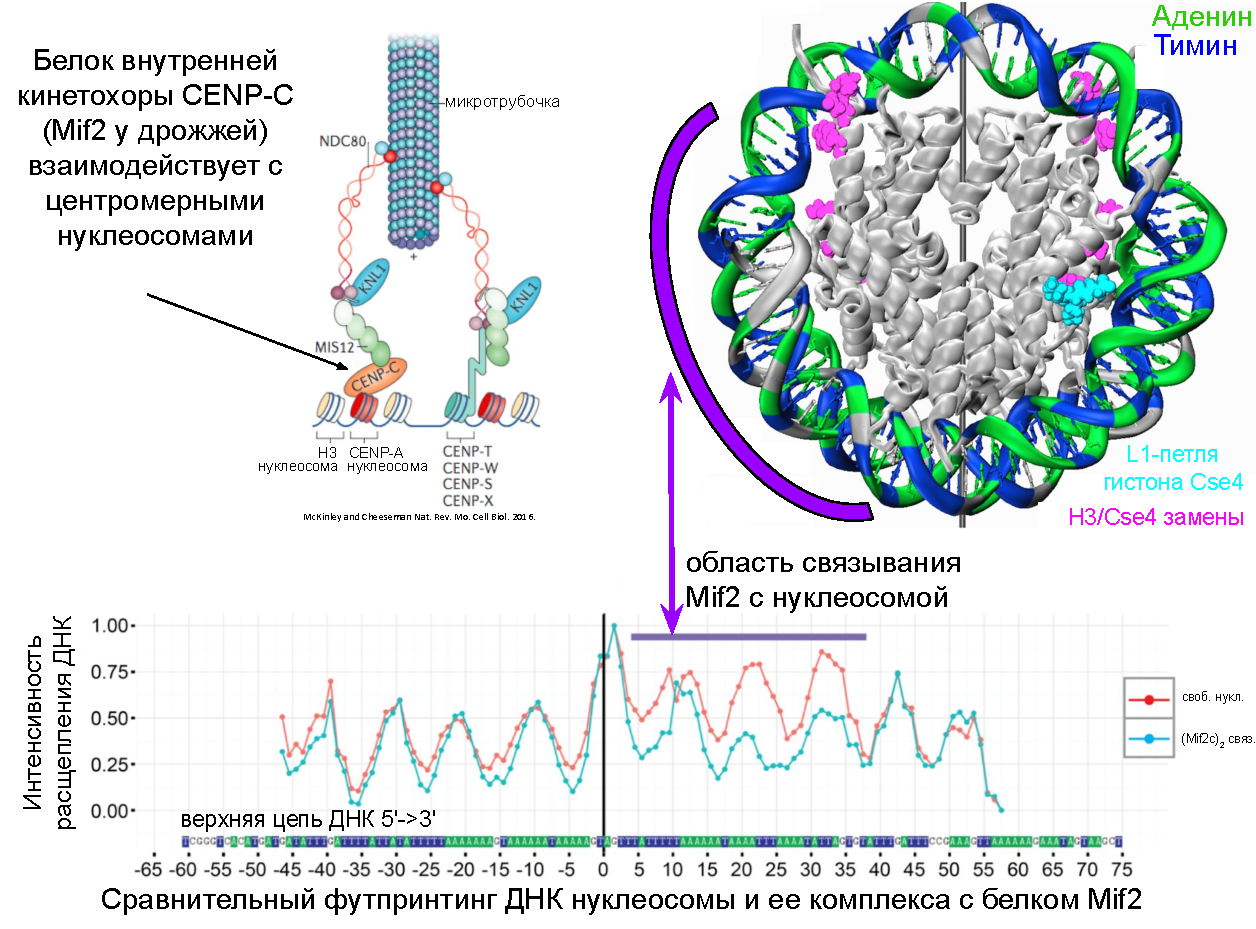
\includegraphics[height=0.9\textheight]{s20}
%\footfullcite{valieva_large-scale_2016}

\note{Метод гидроксильного футпринтинга также можно применять для изучения структуры комплексов нуклеосом с белками. На слайде ранее обсуждавшаяся построенная нами модель центромерной нуклеосомы пекарских дрожжей. С этой нуклеосомой взаимодействет белок CENP-C, который участвует в креплении центромеры к микротрубочкам. Сравнительная обработка экспериментов по футпринтингу чистых нуклеосом и нуклеосом в комплексе с этим белком позволила определить область связывания данного белка с нуклеосомой, отмеченную на рисунке. Как видно из ассиметрии профилей, особенности сиквенса ДНК и его позиционирования оказывают важными для связывания белка с одной стороны нуклеосомы, хотя существует и другая псевдосимметричная сторона.(1-29.5)}
\end{frame}


\section[Глава 5]{Глава 5. Интегративное моделирование амилоидоподобных фибрилл.}

\begin{frame}
\frametitle{Проблема понимания структуры амилоидных фибрилл}
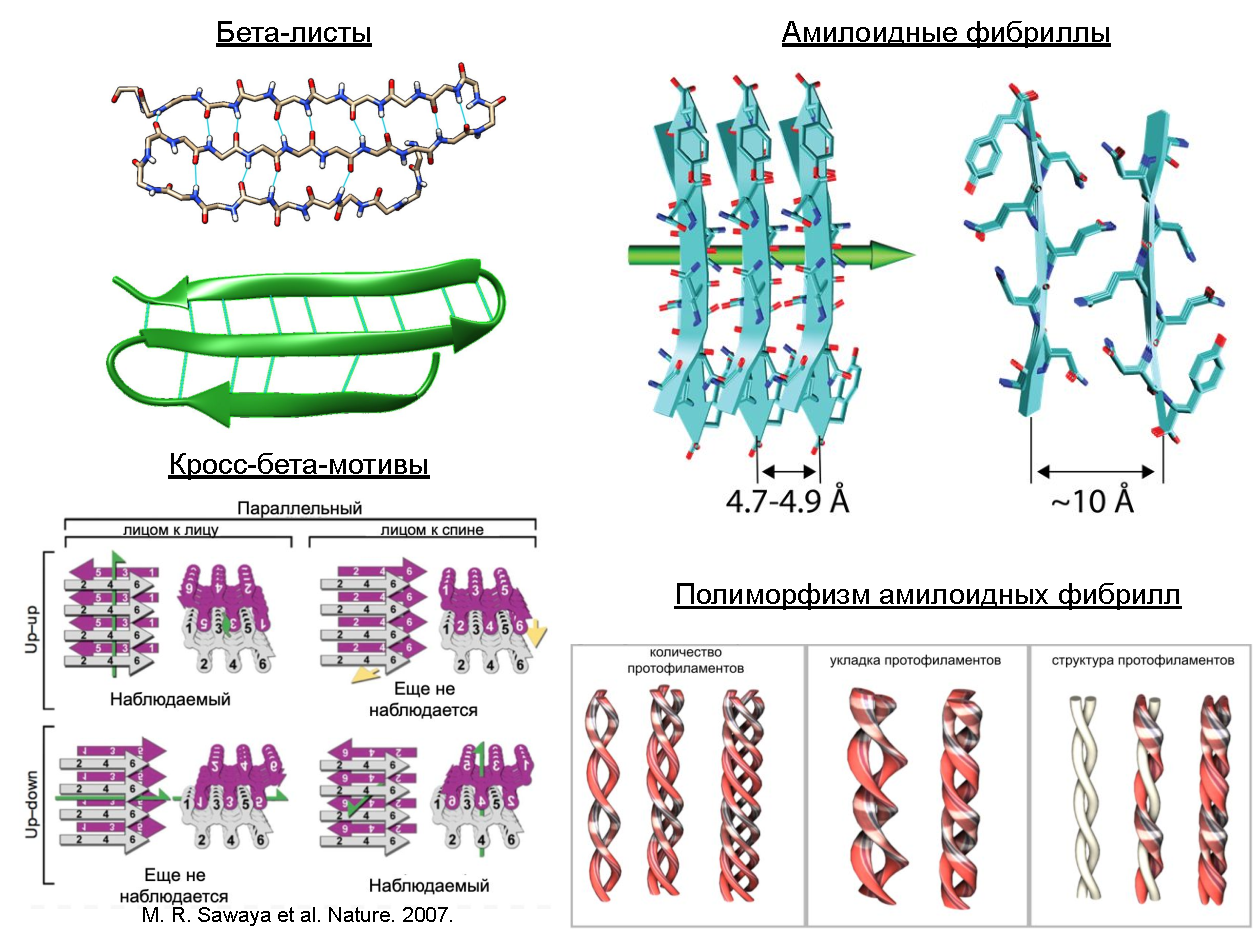
\includegraphics[height=0.9\textheight]{s21}
\note{В последней главе нами рассмотрены методы интегративного моделирвоания в применении к реконструкции амилоидоподобных фибрилл. Амилоидные фибриллы это комплексы, которые собираются из фрагментов белков или их пептидов путем их укладки в длинные бета-листы. Характерным является также взаимодействие бета-листов своими плоскостями и формирование так называемого кросс-бета-мотива, для которого характерна определенная периодичность видимая в экспериментах по рентгеновскому рассеянию. Важной особенностью фибрилл является их полиморфизм, как на уровне различных укладок бета-листов, так и на уровне агрегации и взаимодействия протофиломентов в более крупные фибриллы. Все это приводит к сложности в понимании структуры и свойств амилодоподобных фибрилл.(1-30.5)}
\end{frame}

\begin{frame}
\frametitle{Интегративный подход к моделированию фибрилл}
\centering
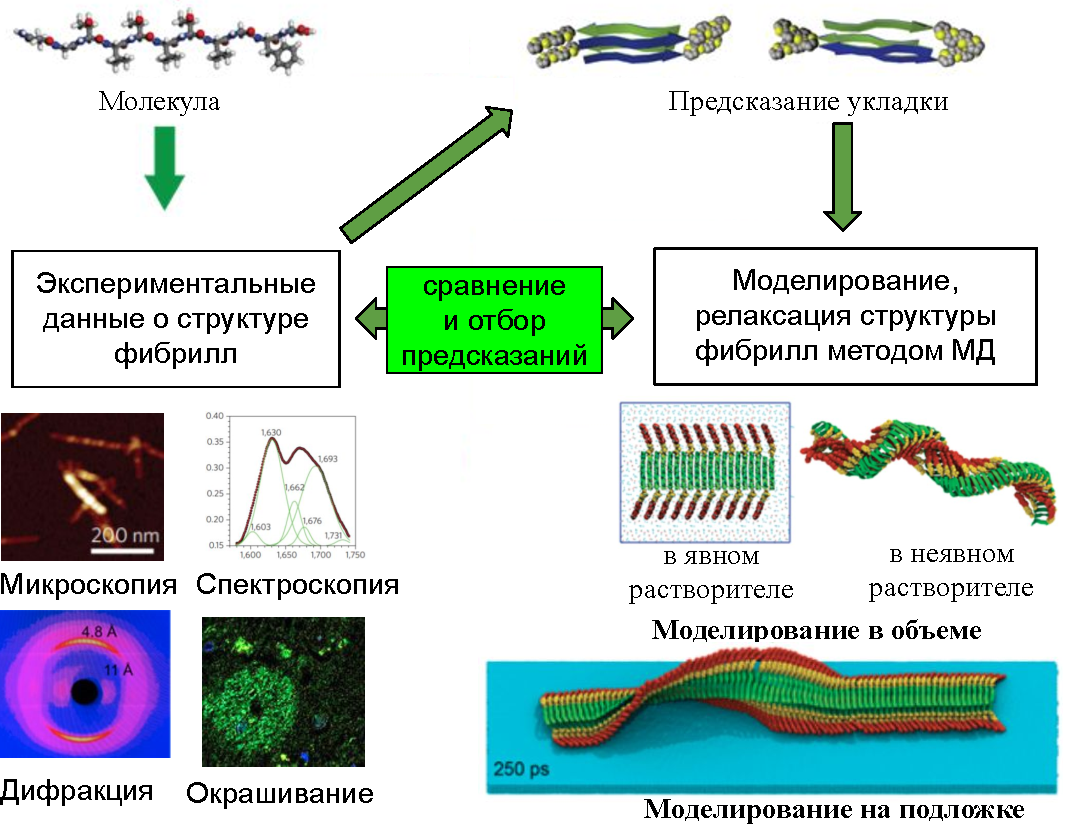
\includegraphics[height=0.85\textheight]{s22}
\note{Нами был предложен и разработан следующий интегративный подход. По экспериментальным данным с учетом различных методов молекулярного моделирования осуществляется предсказание возможных периодических укладок пептидов в фибриллах. К экспериментальным данным могут относится данные КД, ИК спектроскопии, рентгеновской дифракции и т.д. Затем на основе этих укладок конструируются модели фибрилл и проводится их релаксация и расчет методами МД в различных условиях. В результате фибриллы принимают свойственную им крупномасшатбную морфологию, которая стравнивается с данными микроскопии. (1-31.5)}
\end{frame}

\begin{frame}[allowframebreaks]
\frametitle{Нанопровода на основе амилоидоподобных фибрилл}
\centering
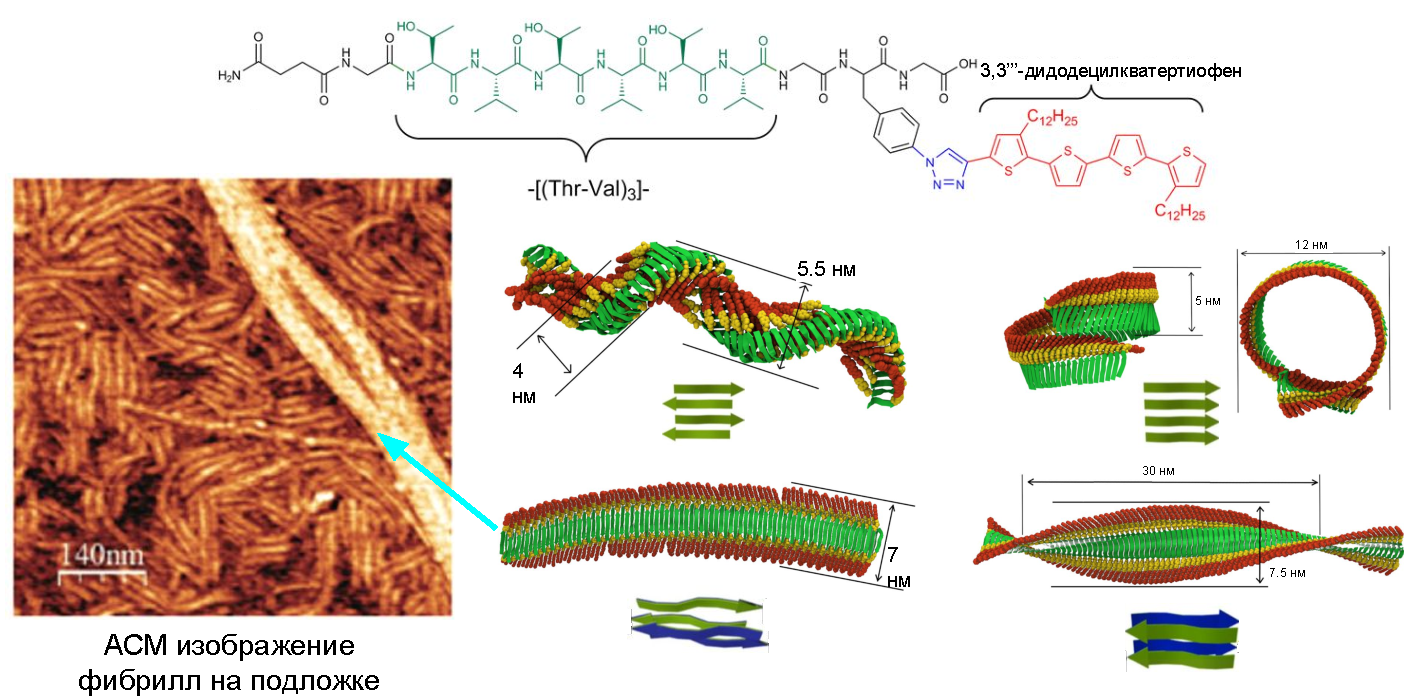
\includegraphics[width=1.0\textwidth]{s23}
\begin{center}
\ifdefined\HANDOUT
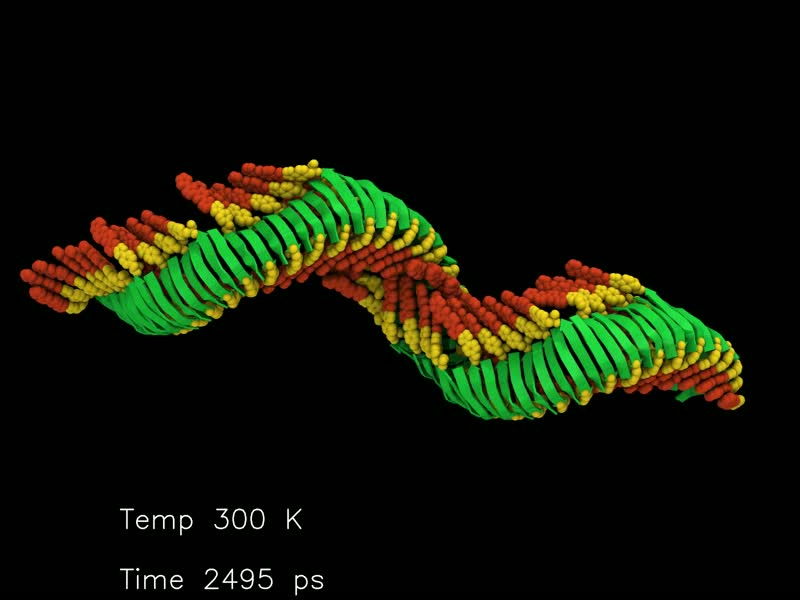
\includegraphics[height=0.75\textheight]{SL-AP/SL-AP500}
\else
\animategraphics[autoplay,height=0.75\textheight,every=2]{10}{SL-AP/SL-AP}{1}{500}
\fi\\
Релаксация начальной модели фибриллы методом МД. Температура поддерживается с помощью метода диссипативной динамики частиц.
\end{center}
\note{Такой подход был нами применен для выяснения структуры и дизайна фибрилл на основе гибридного соединения, состоящего из пептида и проводящего полимера тиофена. На слайде изображены различные укладки и соответвующие им морфологии, полученные в результате моделирования. В результате путем сопоставления изображений атомно-силовой микроскопии и моделей была выбрана наиболее вероятная укладка соответствующая двум анитипараллельным бета-листам, взаимодействующим своими гидрофобными поверхностями. На видео на этом слайде изображен процесс релаксации одной из начальных структур фибрилл. Для плавной резлаксации больших структур был разработан подход, основанный на поддержании постоянной температуры и моделировании неявного растоврителя с помощью метода диссипативной динамики частиц. (1.5-33)}
\end{frame}

\begin{frame}
\frametitle{Фибриллы EF-C из белка gp120}
\centering
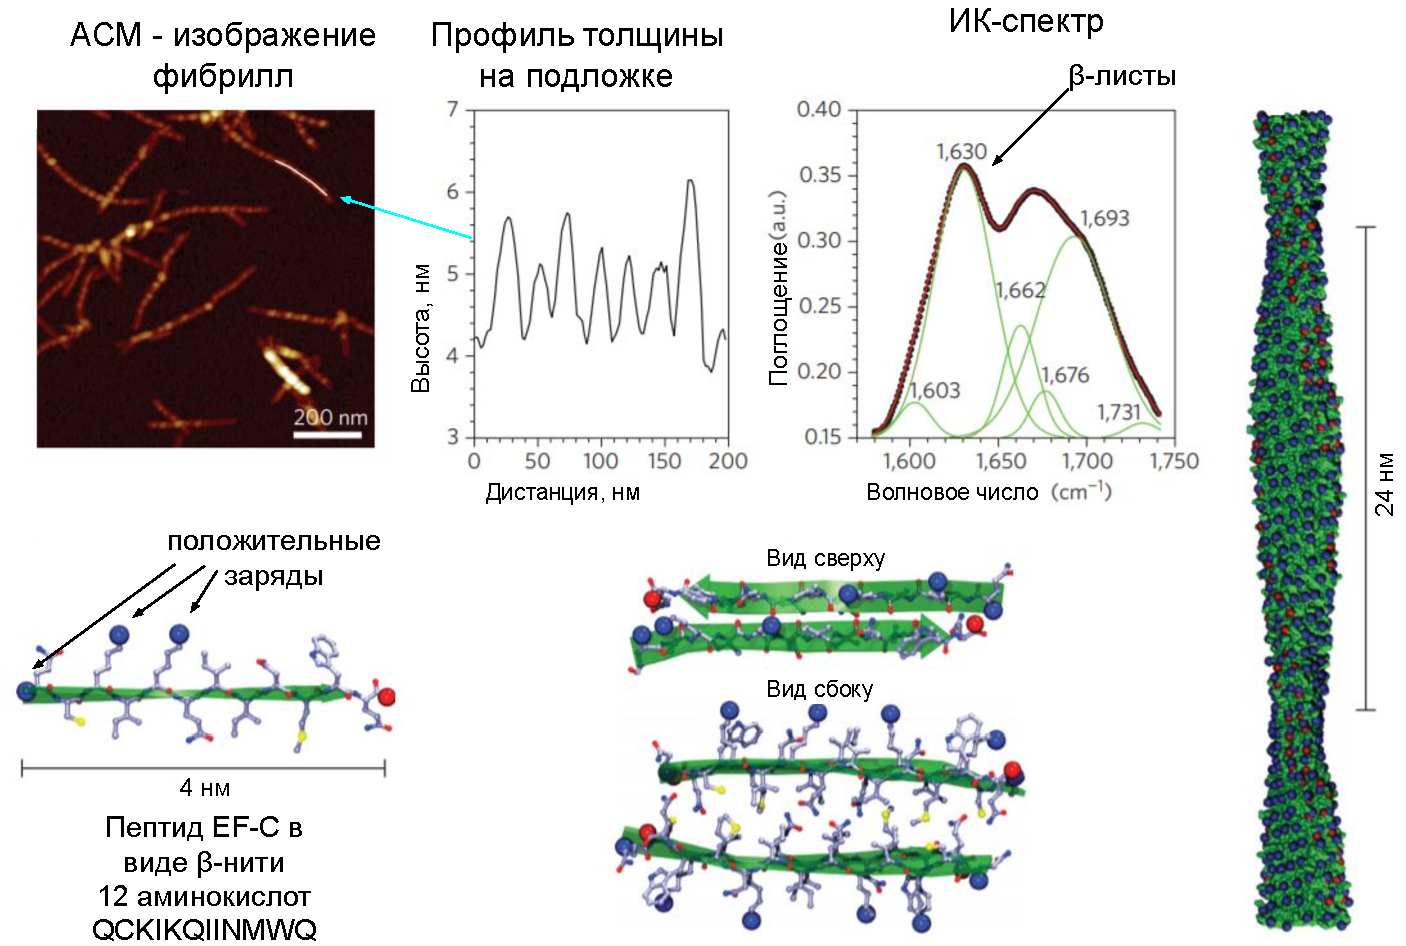
\includegraphics[height=0.85\textheight]{s24}
\note{Похожая задача была нами решена для построения стуруктуры фибрилл из пептидов, названных EF-C. Данные пептиды были выделены, как часть сиквенса гликопротеина gp120 ВИЧ-1. Экспериментально было установлено, что наличие данного пептида приводит к увеличению инфицирования клеток вирусом до 34 раз. На основе данных атомно-силовой микроскопии, кругового дихроизма, инфракрасной спектроскопии, порошковой дифракции рентгеновских лучей с применением разработанного нами интегративного подхода была построена молекулярная модель фибрилл EF-C. Установлено, что боковые цепи лизина образуют гидрофильную поверхность с высокой плотностью катионных зарядов при физиологическом pH. Таким образом фибриллы способствуют взаимодействию отрицательно заряженных поверхностей мембран вирусов с клетками, усиливая проникновение генетического материала вируса в клетку. (1.5-34.5)}
\end{frame}


%   \begin{frame}
% \frametitle{explanation}
% \begin{columns}
% \begin{column}{0.5\textwidth}
%    some text here some text here some text here some text here some text here
% \end{column}
% \begin{column}{0.5\textwidth}  %%<--- here
%     \begin{center}
     
%      \end{center}
% \end{column}
% \end{columns}
% \end{frame}



% \section{Списки}
% \begin{frame}[plain, noframenumbering]
%     \begin{center}
%         \Huge
%         Списки
%     \end{center}
% \end{frame}

% \subsection{Нумерованные}

% \begin{frame}
%     \frametitle{Нумерованные списки}
%     \begin{enumerate}
%         \item один
%         \item два
%         \item три
%     \end{enumerate}
% \end{frame}
% \note{
%     Этот текст будет виден только если его отображение включено
%     в~файле \textbf{Presentation/setup}.
%     Для раздельного вывода презентации и заметок на~разные экраны (как
%     в~impress или powerpoint) можно использовать программу
%     \textit{pdf-presenter-console}.
% }

% \subsection{Не нумерованные}


% \begin{frame}
%     \frametitle{Перечисления}
%     \begin{itemize}
%         \item Проблема 1
%         \item Проблема 2
%         \item Проблема 3
%     \end{itemize}
% \end{frame}
% \note[itemize]{
%     \item Тезис 1
%     \item Тезис 2
%     \item Тезис 3
% }

% \subsection{Комбинированные}

% \begin{frame}
%     \frametitle{Комбинация списков}
%     \begin{enumerate}
%         \item \textbf{Задача 1}
%               \begin{itemize}
%                   \item Подзадача 1-1
%                   \item Подзадача 1-2
%               \end{itemize}
%         \item \textbf{Задача 2}
%               \begin{itemize}
%                   \item Подзадача 2-1
%                   \item Подзадача 2-2
%                   \item Подзадача 2-3
%               \end{itemize}
%         \item \textbf{Задача 3}
%               \begin{itemize}
%                   \item Подзадача 3-1
%                   \item Подзадача 3-2
%                   \item Подзадача 3-3
%               \end{itemize}
%     \end{enumerate}
% \end{frame}
% \note[itemize]{
%     \item Задача 1
%     \item Задача 2
%     \item Задача 3
% }

% \begin{frame}[allowframebreaks]
%     \frametitle{Разделение слайда}
%     Поясняющий текст
%     \begin{itemize}
%         \item Один
%         \item Два
%         \item Три
%     \end{itemize}
%     \framebreak
%     Продолжение предыдущего слайда
% \end{frame}

% \section{Графика}
% \begin{frame}[plain, noframenumbering]
%     \begin{center}
%         \Huge
%         Графика
%     \end{center}
% \end{frame}


% \begin{frame}
%     \frametitle{Одиночное изображение}
%     \centering
%     
\includegraphics[width=0.8\linewidth]{latex} % окружение figure не требуется
% \end{frame}

% \begin{frame}
%     \frametitle{Векторная графика}
%     \begin{figure}
% 	    \centering
% 	    \ifdefmacro{\tikzsetnextfilename}{\tikzsetnextfilename{tikz_presentation}}{}% присваиваемое предкомпилированному pdf имя файла (не обязательно)
% 	    \begin{tikzpicture}
  \draw[<->,thick] (0,6) -- (0,0) -- (10,0); % axis
  \draw[help lines] (3,0) -- (3,5); % fill end
  \draw[help lines] (6,0) -- (6,5); % flattop end
  \draw[help lines] (9,0) -- (9,5); % decay end
  \draw[<->, thin] (0,5) -- (3,5); % fill
  \draw[<->, thin] (3,5) -- (6,5); % flattop
  \draw[<->, thin] (6,5) -- (9,5); % decay
  \draw[blue, ultra thick] (0,0) -- (0,4) -- (6,4) -- (6,0); % power
  \draw[red, ultra thick, domain=0:3] plot (\x, {4*(1 - exp(-1.5*\x))}); % fill plot
  \draw[red, ultra thick, domain=3:6] plot (\x, {4*(1 - exp(-1.5*\x))}); % flattop plot
  \draw[red, ultra thick, domain=6:9.5] plot (\x, {4*(1 - exp(-9)) - 4*(1 - exp(-1.5*\x+9))}); % decay plot
  \node [above] at (0,6) {\(E_{acc}\)};
  \node [right] at (10,0) {\(t\)};
  \node at (1.5,5.4) {заполнение};
  \node at (4.5,5.4) {работа};
  \node at (7.5,5.4) {затухание};
  \node at (4.5,1.4) {пучки};
  \foreach \x in {3.1,3.3,...,5.9} {
    \draw[->, green, thick] (\x,0) -- (\x,1);
  }
\end{tikzpicture}
%     \end{figure}
% \end{frame}

% \subsection{Расположение}

% \begin{frame}
%     \frametitle{Изображения по-вертикали}
%     \centering
%     \vfill
%     
\includegraphics[width=0.8\linewidth,height=0.1\textheight]{latex} \\
%     \TeX
%     \vfill
%     
\includegraphics[width=0.8\linewidth,height=0.2\textheight]{latex} \\
%     \LaTeX
%     \vfill
%     
\includegraphics[scale=0.2]{latex} \\
%     \vfill
% \end{frame}


% \begin{frame}
%     \frametitle{Изображения по-горизонтали}
%     \begin{minipage}[t]{0.47\linewidth}
%         \textbf{Составная \\ подпись 1}
%         \center{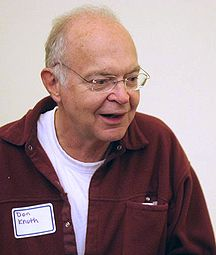
\includegraphics[width=1\linewidth]{knuth1}}
%     \end{minipage}
%     \hfill
%     \begin{minipage}[t]{0.47\linewidth}
%         \textbf{Составная \\ подпись 2}
%         \center{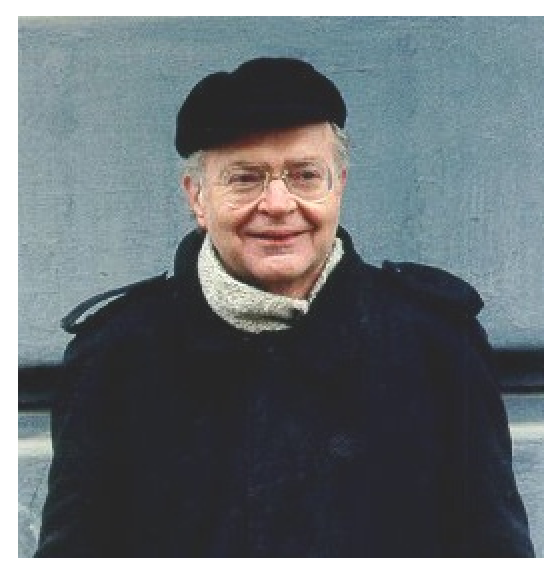
\includegraphics[width=1\linewidth]{knuth2}}
%     \end{minipage}
% \end{frame}

% \subsection{Линии}

% \begin{frame}
%     \frametitle{Разделяющие линии}
%     \begin{minipage}[c]{0.47\linewidth}
%         \center{
\includegraphics[width=1\linewidth]{latex}}
%         \bigskip
%         \hrule{}
%         \bigskip
%         \textbf{Составная \\ подпись 1}
%     \end{minipage}
%     \hfill
%     \vrule{}
%     \hfill
%     \begin{minipage}[c]{0.47\linewidth}
%         \flushright
%         \textbf{Составная \\ подпись 2}
%         \center{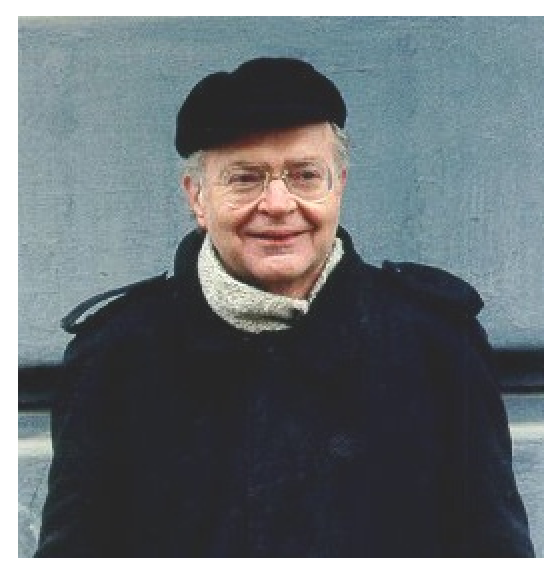
\includegraphics[width=1\linewidth]{knuth2}}
%     \end{minipage}
% \end{frame}

% \section{Остальное}
% \begin{frame}[plain, noframenumbering]
%     \begin{center}
%         \Huge
%         Остальное
%     \end{center}
% \end{frame}

% \subsection{Формулы}

% \begin{frame}
%     \frametitle{Формулы}
%     \[
%     \left\{
%     \begin{array}{rl}
%         \dot x = & \sigma (y-x)  \\
%         \dot y = & x (r - z) - y \\
%         \dot z = & xy - bz
%     \end{array}
%     \right.
%     \]
% \end{frame}

% \begin{frame}
%     \frametitle{amsmath}
%     \centering
%     \begin{minipage}[t]{0.5\linewidth}
%         \begin{multline*}
%             y = 1 x^1 + 2 x^2 + 3 x^3 + \\ + 4 x^4 + 5 x^5 + \dots
%         \end{multline*}
%     \end{minipage}
% \end{frame}

% \begin{frame}[allowframebreaks]
%     \frametitle{Уравнения Максвелла}
%     \centering{
%         \small
%         \def\arraystretch{1.8}%
%         \begin{tabular}{ll}
%             \toprule
%             Интегральная форма                                                                                                                                          & Дифференциальная форма                                                        \\ \midrule
%             \(Q_e(t) = \displaystyle\oiint_S \vec D(t) \cdot d\vec{s} = \displaystyle\iiint_V \rho_v(t) dv\)                                                              & \(\nabla \cdot \vec D(t) = \rho_v(t)\)                                          \\
%             \(\displaystyle\oiint_S \vec B(t) \cdot d\vec{s} = 0\)                                                                                                        & \(\nabla \cdot \vec B(t) = 0\)                                                  \\
%             \(V_{emf}(t) = \displaystyle\oint_L \vec E(t) \cdot d\vec{l}\) = \(- \displaystyle\iint_S \left[\frac{\partial\vec{B}(t)}{\partial t}\right] \cdot d\vec{s}\)   & \(\nabla \times \vec E(t) = - \frac{\partial\vec{B}(t)}{\partial t}\)           \\
%             \(I(t) = \displaystyle\oint_L \vec H(t) \cdot d\vec{l} = \displaystyle\iint_S \left[\vec J(t) + \frac{\partial\vec{D}(t)}{\partial t}\right] \cdot d\vec{s}\) & \(\nabla \times \vec H(t) = \vec J(t) + \frac{\partial\vec{D}(t)}{\partial t}\) \\ \midrule
%             \(\displaystyle\oiint_S \vec J \cdot d\vec{s} = -\frac{\partial Q_e}{\partial t}\)                                                                            & \(\nabla \cdot \vec J = - \frac{\partial \rho_v}{\partial t}\)                  \\
%             \bottomrule
%             \multicolumn{2}{c}{\(\vec D(t) = \left[\varepsilon(t)\right] * \vec E(t)\)}                                                                                                                                                                   \\
%             \multicolumn{2}{c}{\(\vec B(t) = \left[\mu(t)\right] * \vec H(t)\)}                                                                                                                                                                           \\
%         \end{tabular}
%     }
%     \framebreak

%     \hspace{0.05\linewidth}
%     \centering{
%         \small
%         \def\arraystretch{1.8}%
%         \begin{tabular}{ll}
%             \toprule
%             Интегральная форма                                                                                                            & Дифференциальная форма                             \\ \midrule
%             \(Q_e = \displaystyle\oiint_S \vec D \cdot d\vec{s} = \displaystyle\iiint_V \rho_v dv\)                                         & \(\nabla \cdot \vec D = \rho_v\)                     \\
%             \(\displaystyle\oiint_S \vec B \cdot d\vec{s} = 0\)                                                                             & \(\nabla \cdot \vec B = 0\)                          \\
%             \(V_{emf} = \displaystyle\oint_L \vec E \cdot d\vec{l}\) = \(- \displaystyle\iint_S \left[j \omega \vec B\right] \cdot d\vec{s}\) & \(\nabla \times \vec E = - j \omega \vec B\)         \\
%             \(I = \displaystyle\oint_L \vec H \cdot d\vec{l} = \displaystyle\iint_S \left[\vec J + j \omega \vec D\right] \cdot d\vec{s}\)  & \(\nabla \times \vec H = \vec J + j \omega \vec{D}\) \\ \midrule
%             \(\displaystyle\oiint_S \vec J \cdot d\vec{s} = - j \omega Q_e\)                                                                & \(\nabla \cdot \vec J = - j \omega \rho_v\)          \\
%             \bottomrule
%             \multicolumn{2}{c}{\(\vec D(t) = \left[\varepsilon\right] \vec E(t)\)}                                                                                                               \\
%             \multicolumn{2}{c}{\(\vec B(t) = \left[\mu\right] \vec H(t)\)}                                                                                                                       \\
%         \end{tabular}
%     }
% \end{frame}

% \subsection{Таблицы}

% \begin{frame}
%     \frametitle{Таблица}
%     \centering
%     \begin{tabular}{|l|l|}
%         \hline
%         \textbf{Заголовок 1} & \textbf{Заголовок 2} \\
%         \hline
%         Сумма                & \(b+a\)                \\
%         \hline
%         Разность             & \(a-b\)                \\
%         \hline
%         Произведение         & \(a*b\)                \\
%         \hline
%     \end{tabular}
% \end{frame}

% \begin{frame}
%     \frametitle{Другая таблица}
%     \centering
%     \begin{tabular}{lc}
%         \toprule
%         \multicolumn{1}{c}{\textbf{Заголовок 1}} & \textbf{Заголовок 2} \\ \midrule
%         Сумма                                    & \(b+a\)                \\
%         Разность                                 & \(a-b\)                \\
%         Произведение                             & \(a*b\)                \\
%         \bottomrule
%     \end{tabular}
% \end{frame}


% \subsection{Разное}

% \begin{frame}
%     \frametitle{Большой многоуровневый список}
%     \begin{itemize}
%         \item \textbf{Пункт 1}
%               \begin{itemize}
%                   \itemi Подпункт 1-1
%                   \itemi Подпункт 1-2
%               \end{itemize}
%         \item \textbf{Пункт 2}
%               \begin{itemize}
%                   \itemi Подпункт 2-1
%               \end{itemize}
%         \item \textbf{Пункт 3}
%               \begin{itemize}
%                   \itemi Подпункт 3-1
%                   \itemi Подпункт 3-2
%               \end{itemize}
%         \item \textbf{Пункт 4}
%               \begin{itemize}
%                   \itemi Подпункт 4-1
%               \end{itemize}
%         \item \textbf{Пункт 5}
%               \begin{itemize}
%                   \itemi Подпункт 5-1
%                   \itemi Подпункт 5-2
%                   \itemi Подпункт 5-3
%               \end{itemize}
%     \end{itemize}
% \end{frame}

% \begin{frame}
%     \frametitle{Четыре изображения}
%     \centering
%     
\includegraphics[width=0.35\linewidth,angle=35]{latex}
%     
\includegraphics[width=0.35\linewidth,angle=135]{latex}\\
%     
\includegraphics[width=0.35\linewidth,angle=15]{latex}
%     
\includegraphics[width=0.35\linewidth,angle=-15]{latex}
% \end{frame}

